\documentclass{scrartcl}
\usepackage{cook}

% Schriftarten für Überschriften
\usepackage{aurical}
\usepackage{calligra}
\usepackage{yfonts}
\usepackage{uncial}
\usepackage{rustic}
\usepackage{rotunda}
\usepackage{inslrmin}
\usepackage{pbsi}
\usepackage{egothic}
\usepackage{sqrcaps}
\usepackage{tikz}

\definecolor{darkblue}{rgb}{0,0,.5}
\usepackage[ % muss letztes Package sein!
	pdftitle={Muttis beste Küche - Kochen wie Daheim},%
	pdfauthor={Max Klenk},%
	pdfsubject={Kochbuch},%
	pdfcreator={PDFLaTeX},
	pdfproducer={LaTeX mit Windows 7},
	colorlinks=true, urlcolor=darkblue, linkcolor=darkblue
 ]{hyperref} % 

%\twosided 	% Zweiseitig?

\begin{document}

% entweder die Optionen ausfüllen und mit \maketitle Titelseite erzeugen oder...
%\title{Meine Küche}
%\author{Autor}

% ... die Titelseite selber zusammenstellen
\begin{titlepage}
		\begin{figure}[H]% einfügen der Grafik
			\centering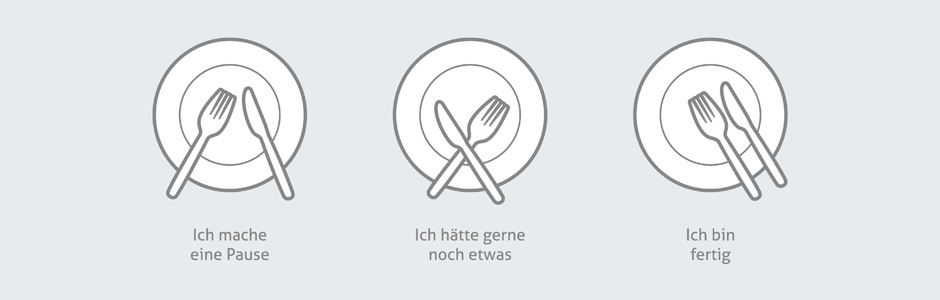
\includegraphics[height=0.5\textheight]{./bilder/start_.jpg} \\
			Muttis beste Küche - Kochen wie Daheim \\
			 \
			 \\
			 \
			 \\
			 \
			 \\
			 \
			 \\
			 \
			 \\
			 \
			 \\
			 \
			 \\
			 \
			 \\
			 \
			 \\
			Bewährte Rezepte gesammelt für Max, Clemens und Lucius (und ein paar Ergänzungen).
		\end{figure}
%\newpage
%\centering\vspace*{3cm}\copyright \ 2012 Max Klenk
\end{titlepage}

\tableofcontents

% Standardfarbe, -schriftart für die Überschrift
\recipecolor{C20E0F}
\recipefont{\texttt}

% wenn \twosided aktiv ist (bei Zweiseitig ist die ungerade Zahl immer auf der Vorderseite)
% müssen hier soviele newpages einfügen bis die erste Sektion auf einer ungeraden Seite beginnt
%\newpage~

\newpage % vor jede Sektion muss ein Newpage kommen
{\vspace*{4cm}\section{Vorspeisen}}
\newpage
\tikz[remember picture,overlay] \node[opacity=1,inner sep=0pt] at (current page.center){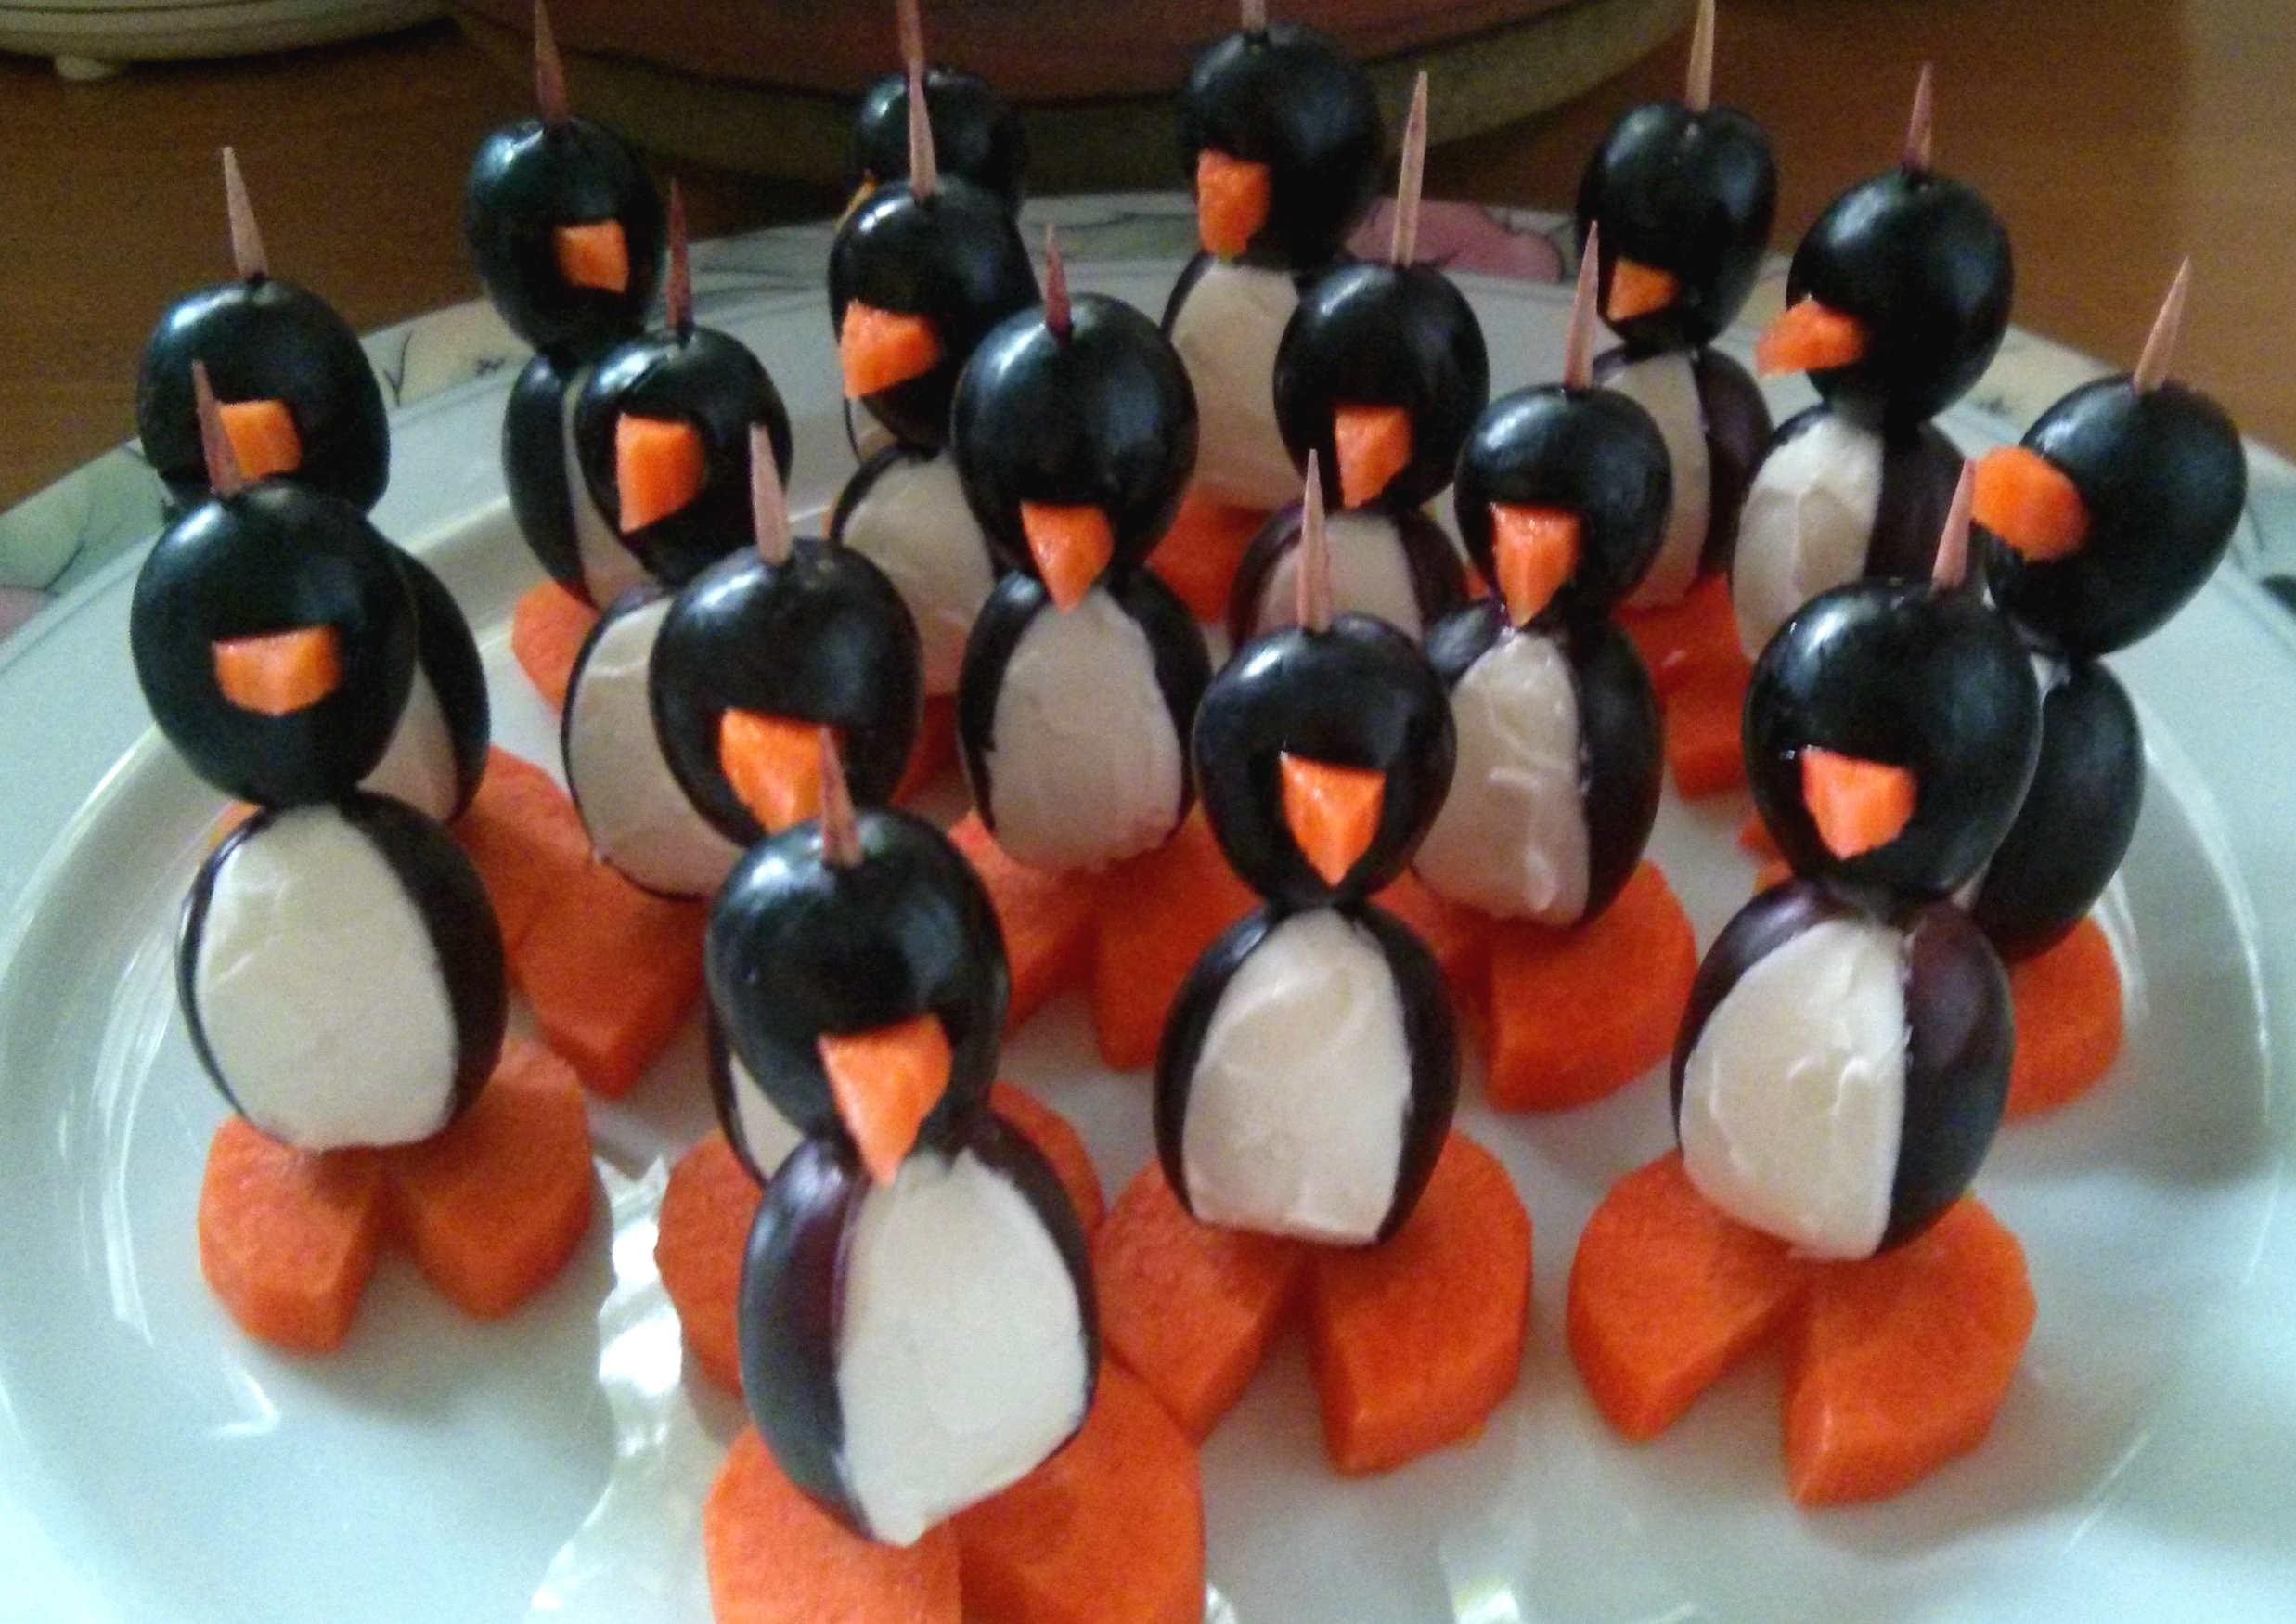
\includegraphics[width=\paperwidth,height=\paperheight]{./bilder/pinguine_ratio.jpg}};

\begin{recipe}[]{Pinguine} %Quelle
	\timerecipe[Minuten]{ca. 30} %mit [EINHEIT]
	\personcount[Stück]{10} % mit[ART]
	\ingredient{1 Karotte} % ggf. \nicefrac{1}{2}
	\ingredient{20 dunkle Weintrauben}
	\ingredient{200g Frischkäse}
	\ingredient{10 Zahnstocher}

\step
\textbf{1 Karotte} in drei bis vier Millimeter dicke Scheibchen schneiden. Aus den Möhrenscheibchen mit je zwei Schnitten bis zur Mitte ein kleines Dreieck herausschneiden. Dreieck beiseitelegen (ergibt den Schnabel des Pinguins). 

\step
In eine \textbf{kleinere rote Traube} einen sehr kleinen Schlitz für den Schnabel schneiden und die Möhrenecke einstecken. Aus einer \textbf{größeren Traube} ein Drittel als Spalte ausschneiden. 

\step
Den entstandenen Spalt sauber mit \textbf{Frischkäse} füllen (das gibt den Pinguinbauch). Die beiden Trauben auf einen Zahnstocher stecken (die kleine als Kopf oben, die große als Bauch unten) und unten die Karotten-Füße befestigen.

%\tippbox{\textbf{Tipp:} ...} % Tipp in extra Rahmen
\end{recipe}

\newpage
{\vspace*{4cm}\section{Salate}}
\ifdefined\withimages
	\newpage
	\tikz[remember picture,overlay] \node[opacity=1,inner sep=0pt] at (current page.center){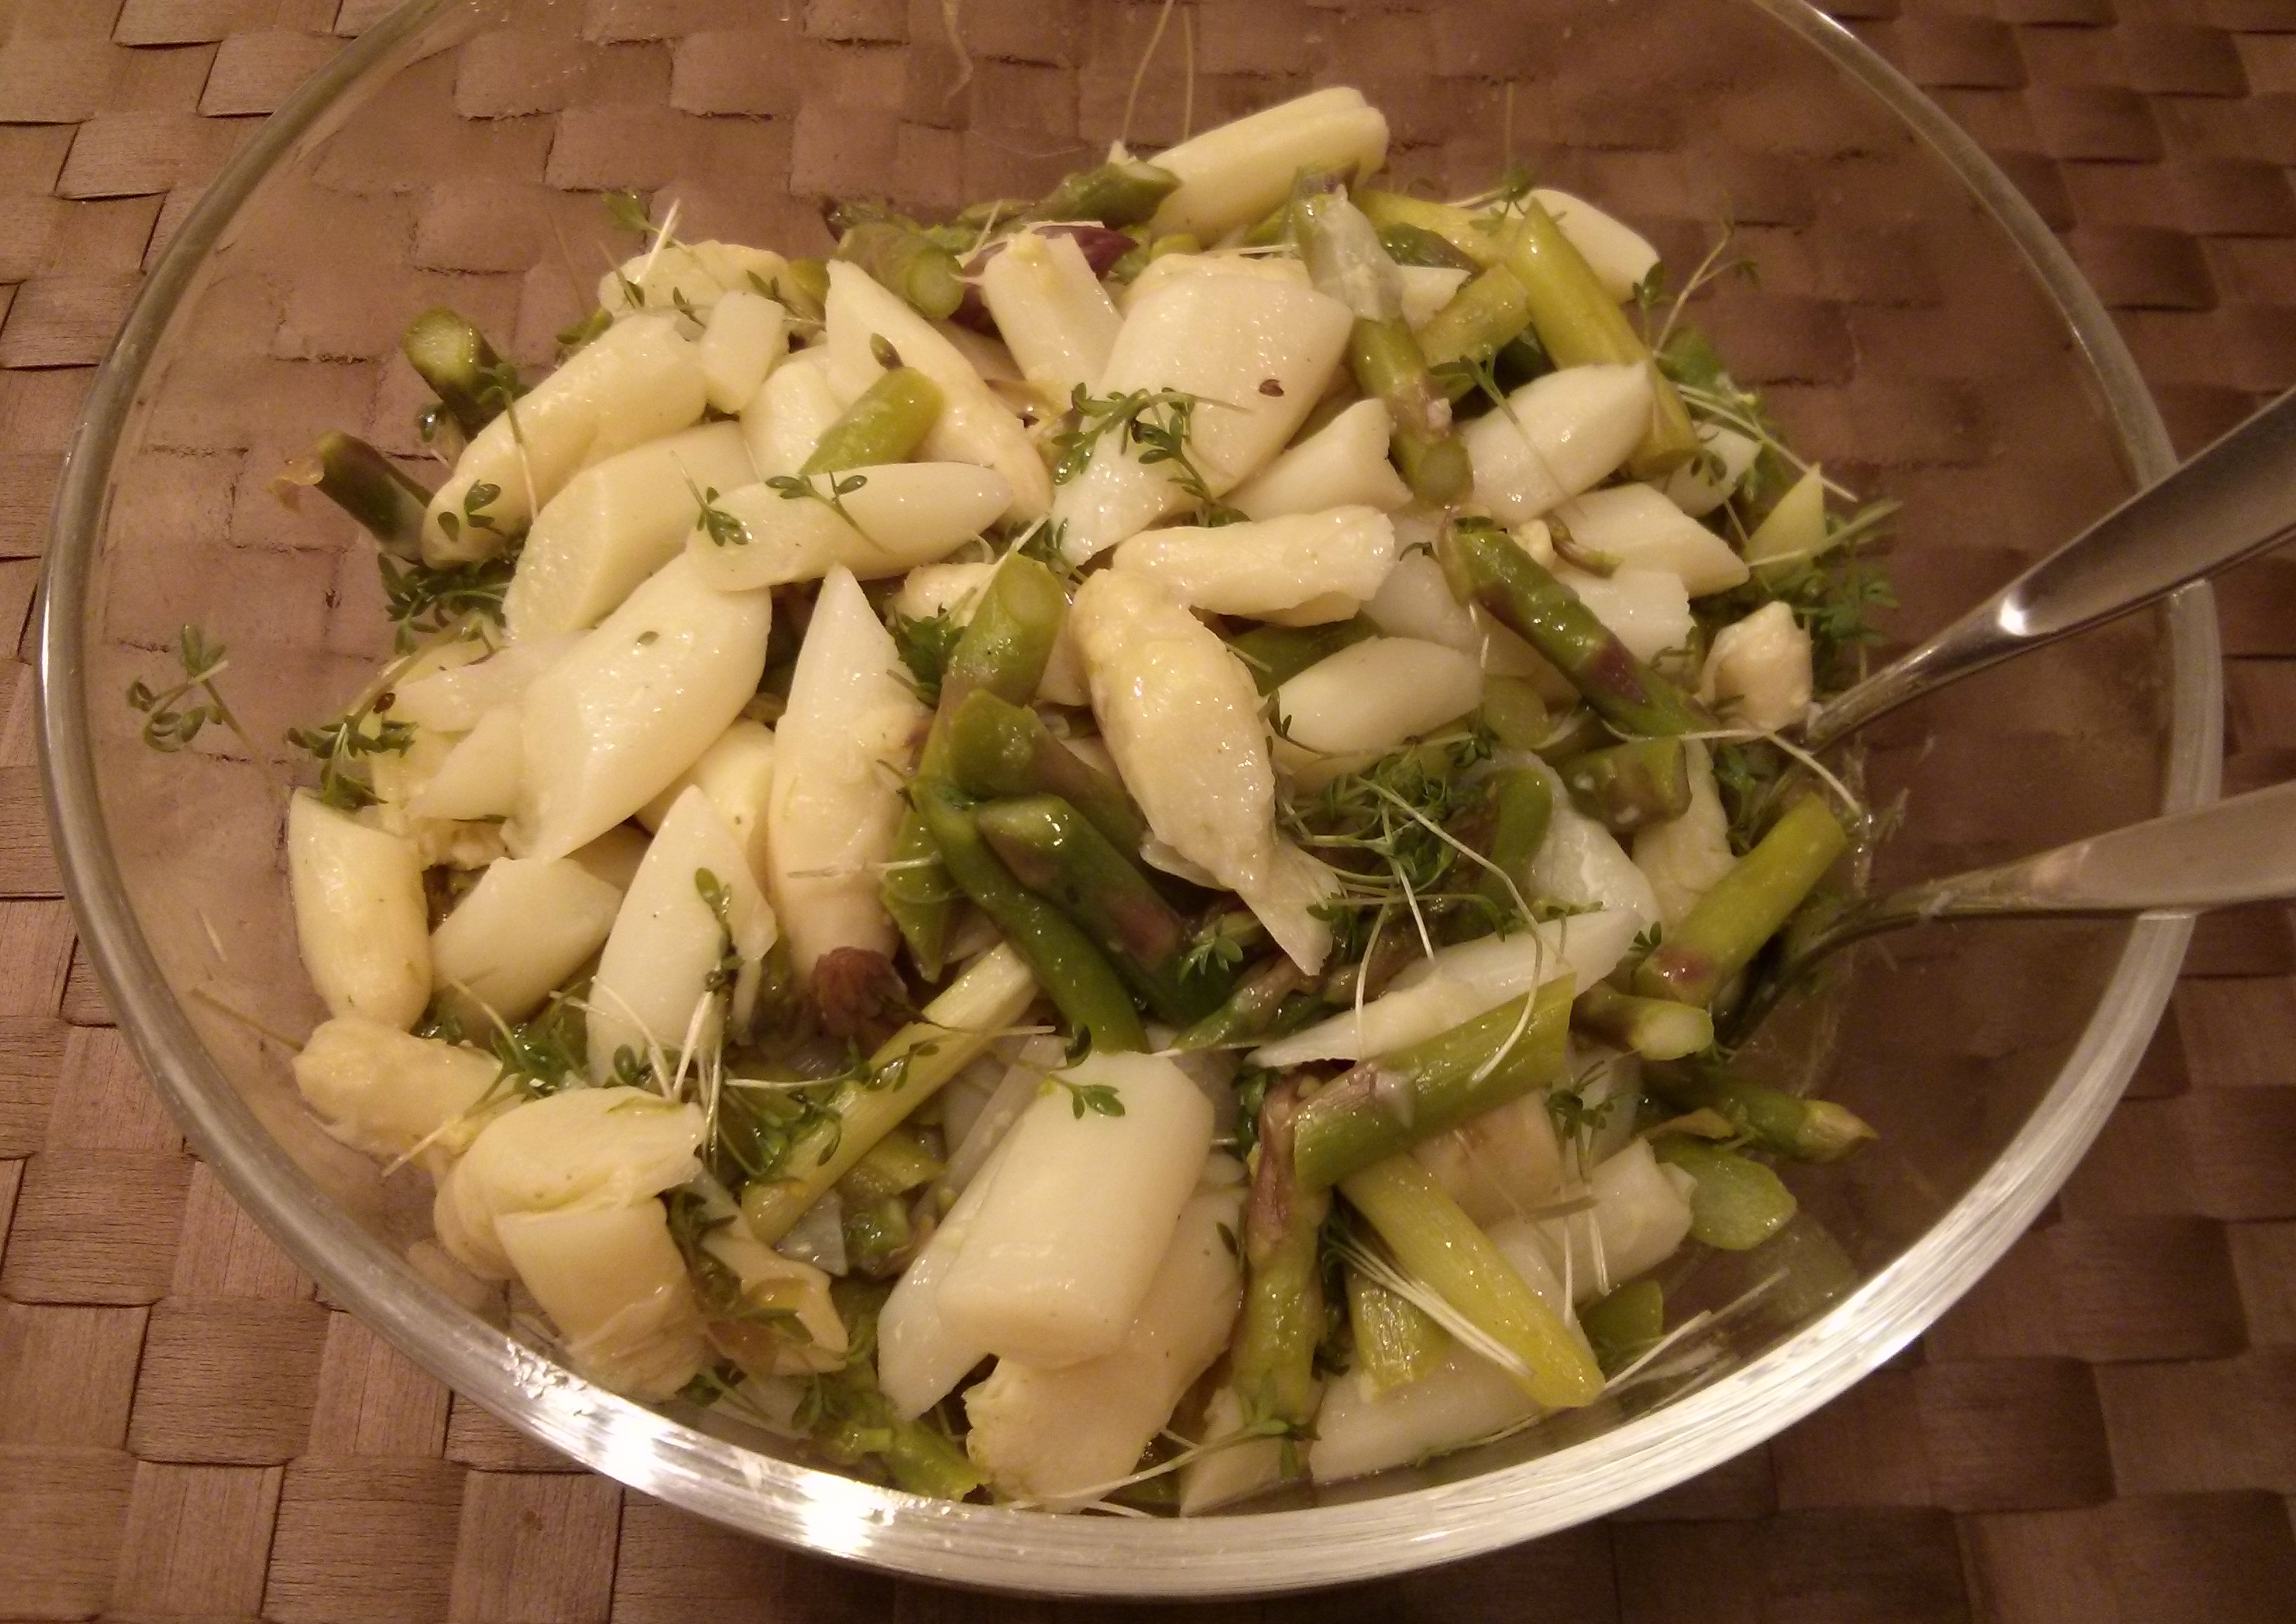
\includegraphics[width=\paperwidth,height=\paperheight]{./bilder/spargelsalat_ratio.jpg}};
\fi

\begin{recipe}[]{Warmer Spargelsalat} %Quelle
	\timerecipe[Minuten]{ca. 30} %mit [EINHEIT]
	\personcount{2} % mit[ART]
	\ingredient{500g Spargel (weiß/grün/gemischt)} % ggf. \nicefrac{1}{2}
	\ingredient{Traubenkernöl}
	\ingredient{weißer Balsamico}
	\ingredient{Brunnenkresse}
	\ingredient{Salz}
	\ingredient{Pfeffer}
	\ingredient{Zucker}
	\ingredient{Zitronensaft}


\step
\textbf{Spargel} schälen (grünen Spargel nur im unteren Drittel) und in 3-4cm lange Stückchen schneiden.

\step
Spargel mit etwas \textbf{Salz}, \textbf{Zucker}, \textbf{Butter} und \textbf{Zitronensaft} im Wasser kochen (grüner Spargel ist schneller gar als weißer, als erst später ins Wasser geben).

\step
Während der Spargel etwas abkühlt aus \textbf{Traubenkernöl}, \textbf{weißem Balsamico}, \textbf{Salz} und \textbf{Pfeffer} eine Salatsoße mischen.

\step
Spargel vorsichtig mit der Salatsoße mischen und die \textbf{Brunnenkresse} darauf drapieren. Lauwarm servieren.

%\tippbox{\textbf{Tipp:} ...} % Tipp in extra Rahmen
\end{recipe}

\newpage
{\vspace*{4cm}\section{Mahlzeit}}
\newpage
\tikz[remember picture,overlay] \node[opacity=1,inner sep=0pt] at (current page.center){\includegraphics[width=\paperwidth,height=\paperheight]{./bilder/gefueltes_brot_ratio.jpg}};


\begin{recipe}[]{Gefülltes Brot} %Josi
	\timerecipe[Minuten]{ca. 15 + 60 + 15 + 30} %mit [EINHEIT]
	\personcount{2-3} % mit[ART]
	\ingredient{300g Mehl} % ggf. \nicefrac{1}{2}
	\ingredient{15g frische Hefe}
	\ingredient{150g gekocheter Schinken}
	\ingredient{1 Bund Petersilie}
	\ingredient{2 Knoblauchzehen}
	\ingredient{1 Kugel Mozzarella}
	\ingredient{50g getrocknete Tomaten}
	\ingredient{1 Eigelb}

\step \textbf{15g Hefe} und \textbf{eine Prise Zucker} in 160ml lauwarmen Wasser lösen und mit \textbf{1\nicefrac{1}{2} EL Olivenöl}, \textbf{1 TL Salz} und \textbf{300g Mehl} zu einen glatten Teig kneten. 

\step Den Teig ca. eine Stunden an einem warmen Ort gehen lasse.

\step Den Backofen auf 200 Grad Ober-/Unterhitze vorheizen.

\step \textbf{150g gekochten Schinken} in Streifen schneiden, \textbf{1 Bund Petersilie} und \textbf{2 Knoblauchzehen} fein hacken und  \textbf{50g getrockneten Tomaten} und \textbf{eine Kugel Mozzarella} würfeln. Mischen und mit \textbf{Salz} und \textbf{Pfeffer} würzen.

\step Den Teig in zwei Fladen ausrollen und auf dem einen die Masse bis an den Rand verteilen. Nun den zweiten Fladen kreuzweise einschneiden und auf dem ersten an drücken und mit \textbf{einem Eigelb} bepinseln.

\step 20-25 Minuten auf mittlerer Schiene backen und noch lauwarm essen.

%\tippbox{{Tipp:} ...} % Tipp in extra Rahmen
\end{recipe}
\newpage
\tikz[remember picture,overlay] \node[opacity=1,inner sep=0pt] at (current page.center){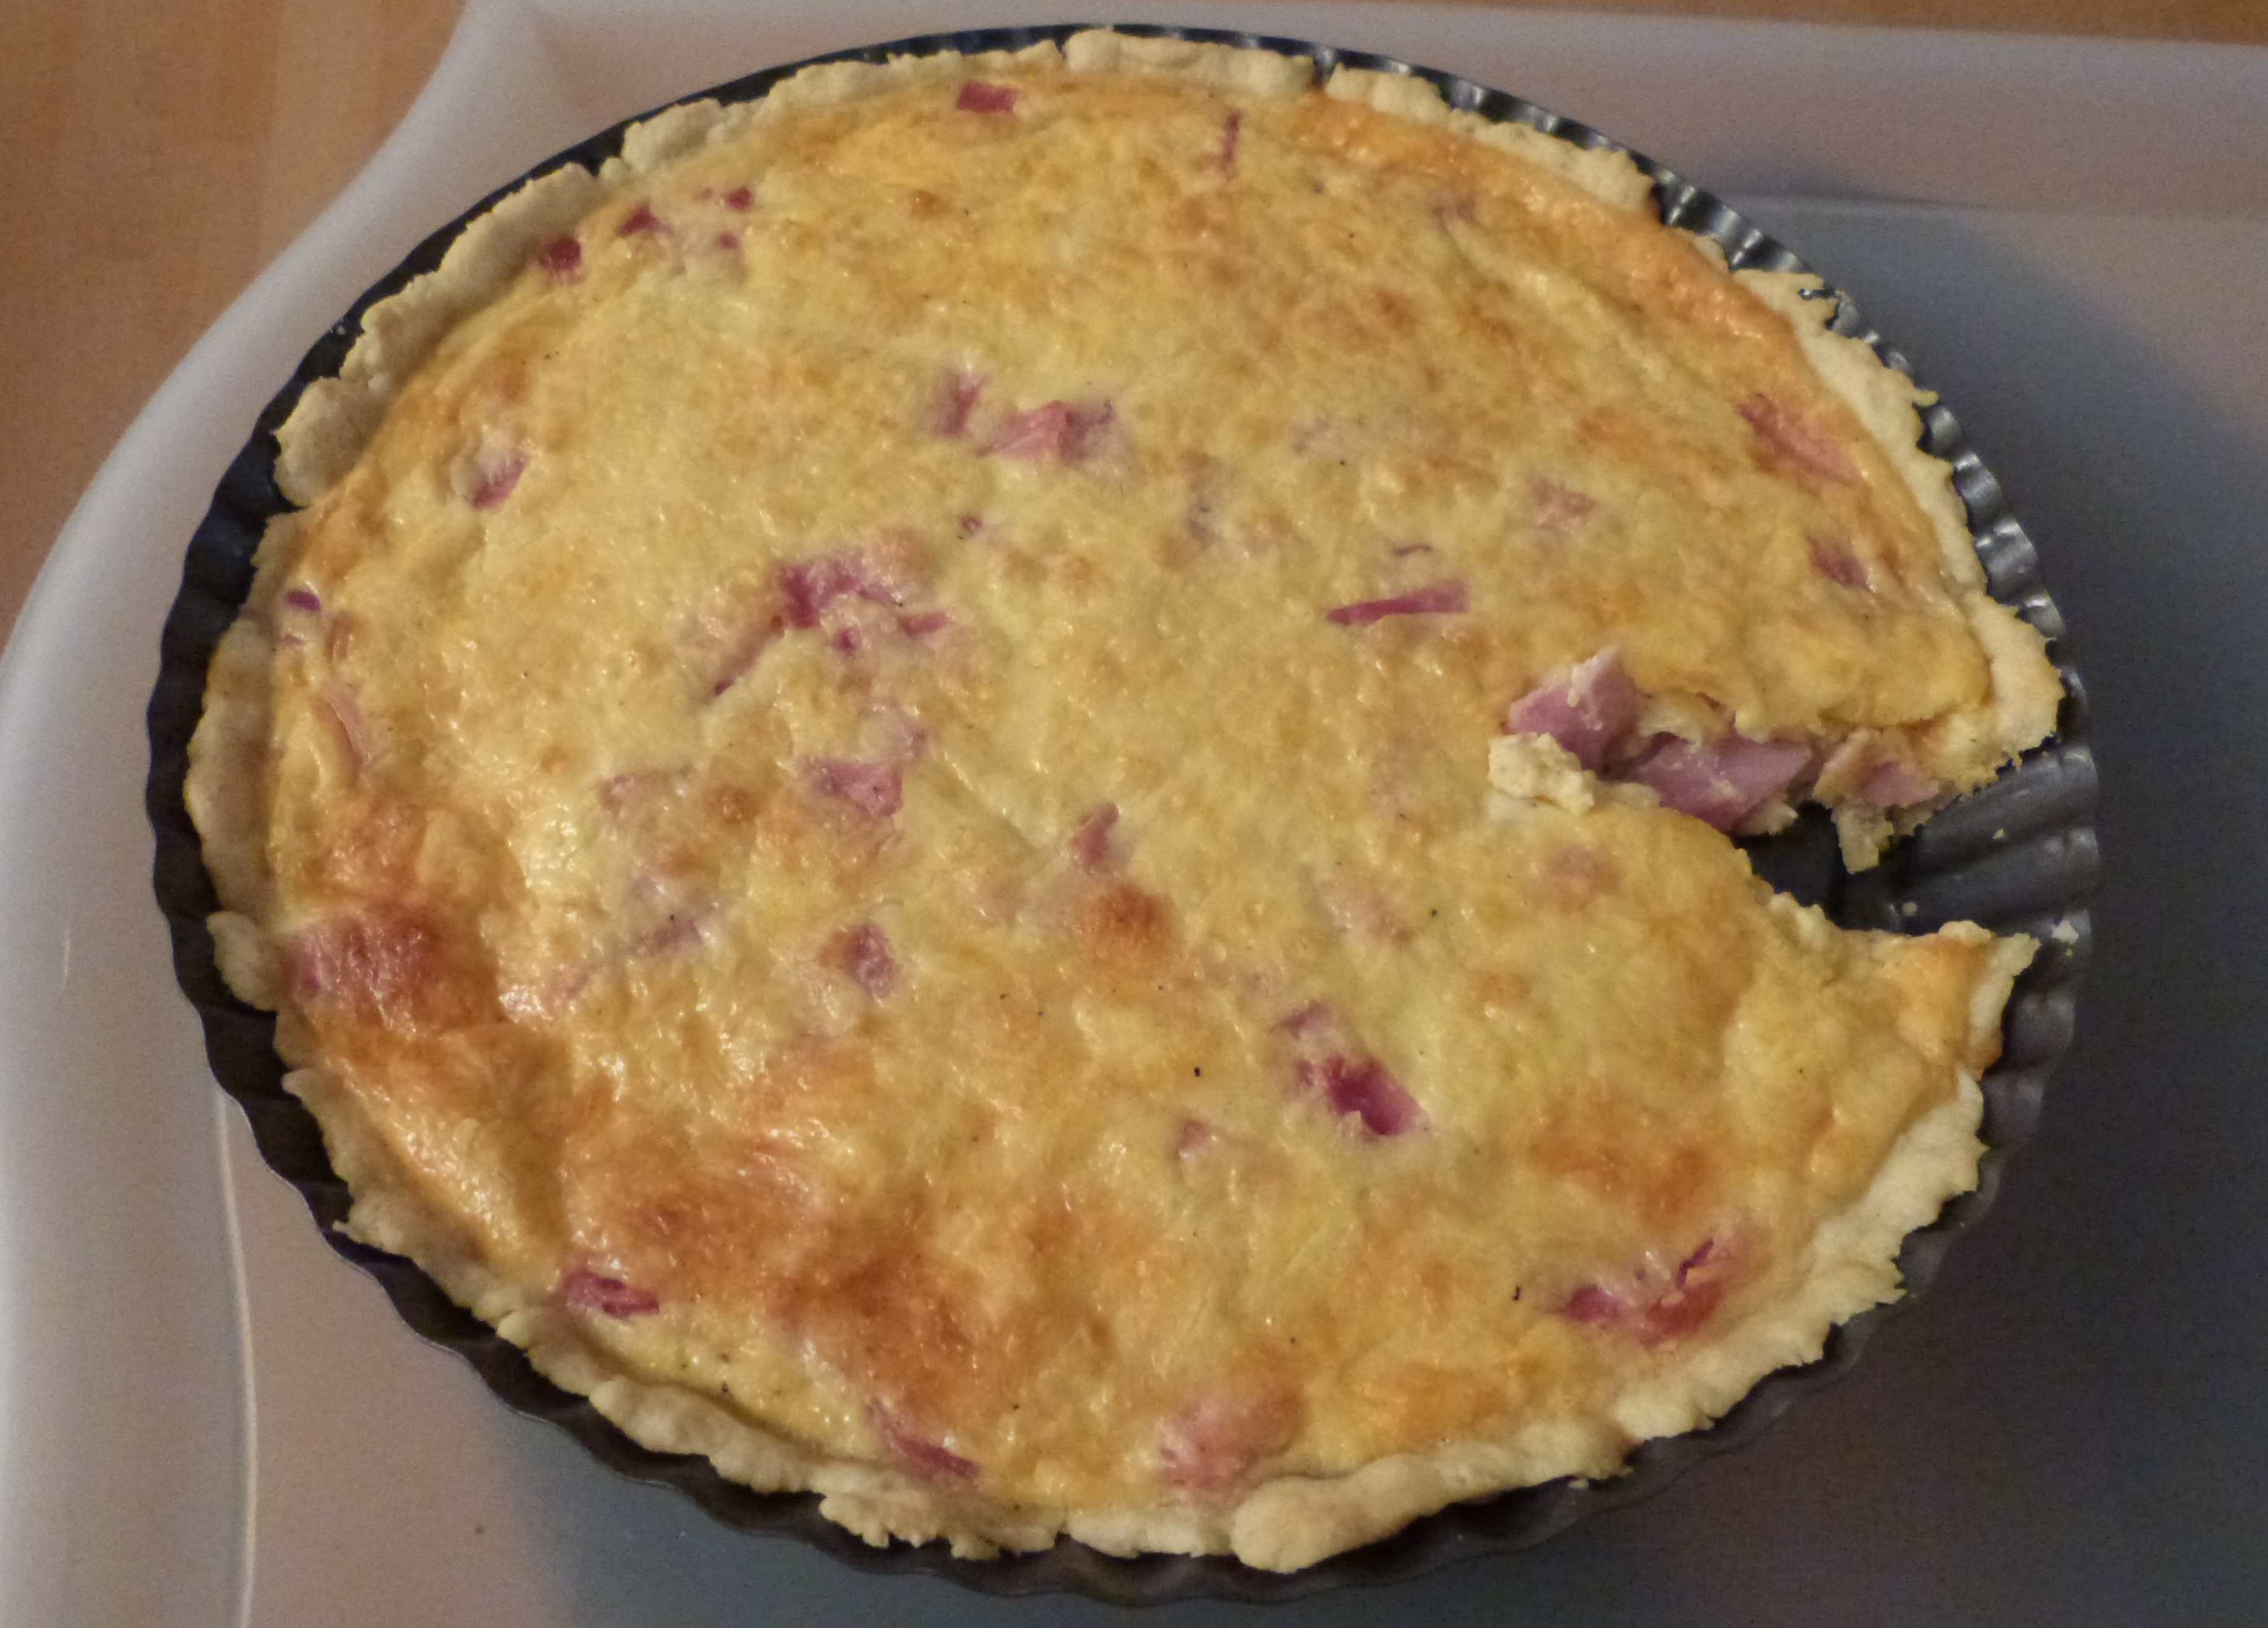
\includegraphics[width=\paperwidth,height=\paperheight]{./bilder/quiche_lorraine_ratio.jpg}};

\begin{recipe}[]{Quiche lorraine} % Mutti Feb 14 
	\timerecipe[Minuten]{ca. (60)+15+30} %mit [EINHEIT]
	\personcount[Personen]{2} % mit[ART]
	\ingredient{200g Mehl} % ggf. \nicefrac{1}{2}
	\ingredient{100g Butter}
	\ingredient{200g gekochter Schinken}
	\ingredient{3 Eier}
	\ingredient{\nicefrac{1}{4} Liter Sahne}
	\ingredient{125g geriebener Emmentaler}


\step
\textbf{200g Mehl}, \textbf{100g Butter}, \textbf{\nicefrac{1}{2} TL Salz} und \textbf{5 EL Wasser} zu einem Teig kneten und 1 Stunde kalt stellen.

\step
Backofen auf 200 Grad vorheizen.

\step
Teig in einer Springform ausrollen und mehrmals mit einer Gabel einstechen.

\step
\textbf{200g Schinken} in Streifen schneiden und auf dem Teig verteilen.

\step
\textbf{3 Eier}, \textbf{\nicefrac{1}{4} Liter Sahne} und \textbf{Pfeffer} verquirlen, die \textbf{125g geriebener Emmentaler} untermischen und auf dem Teig verteilen.

\step
Quiche auf der zweiten Schiene von unten ca. \nicefrac{1}{2} Stunde backen, bis sie eine schöne Farbe hat.


\tippbox{{Tipp:} Statt Schinken kann man auch gewürfelte Zuccinis oder Blattspinat oder in Scheiben geschnittene Champignons nehmen.} % Tipp in extra Rahmen
\end{recipe}
\begin{recipe}[]{Lasagne} %MUTTI Dez
	\timerecipe[Minuten]{ca. ??} %mit [EINHEIT]
	\personcount[Auflaufform]{1} % mit[ART]
	\ingredient{500g Hackfleisch gemischt} % ggf. \nicefrac{1}{2}
	\ingredient{2 Zwiebeln}
	\ingredient{2 Knoblachzehen}
	\ingredient{2-3 Karotten}
	\ingredient{1 Packung passierte Tomaten}
	\ingredient{1 Becher Sahne}
	\ingredient{1 Beute geriebener Käse}
	\ingredient{500g Lasagneplatten}

\step
Ofen auf 180°C Ober-Unterhitze vorheizen.

\step
Soße wir die normale Hackfleischsoße zubereiten.

\step
\textbf{2 EL Butter} in einem Topf schmelzen und mit \textbf{2-3 EL Mehl} verrühren bis es goldgelb ist. Dann \textbf{1 Becher Sahne} unterrühren und aufkochen. Soviel \textbf{Milch} dazugeben, bis die Soße schön flüssig ist. Mit den Gewürzen abschmecken und die \textbf{Hälfte des Käses} darin schmelzen lassen.

\step
Ein Auflaufform einfetten und dann erst Tomatensoße, dann Nudelplatten(einschichtig) und dann die helle Soße schichten. Mehrmals wiederholen, bis die Form voll ist. Die oberste Schicht sollte helle Soße sein. Diese mit dem \textbf{restlichen Käse} bestreuen und 

\step
Bei ca. 180°C Ober-Unterhitze solange backen, bis der Käse geschmolzen ist und Farbe bekommt.





%\tippbox{{\bf Tipp:} ...} % Tipp in extra Rahmen
\end{recipe}
\begin{recipe}[]{Ratatouille} %MUTTI Dez
	\timerecipe[Minuten]{ca. } %mit [EINHEIT]
	\personcount{} % mit[ART]
	\ingredient{2-3 Zucchini} % ggf. \nicefrac{1}{2}
	\ingredient{1 Aubergine}
	\ingredient{1 rote Paprika}
	\ingredient{1 gelbe Paprika}
	\ingredient{400g Tomaten oder Dosentomaten}
	\ingredient{1 große rote Zwiebel}
	\ingredient{4 Knoblauchzehen}
	\ingredient{2-3 Zweige Thymian}
	\ingredient{\nicefrac{1}{2} Bund Basilikum}

\step
\textbf{2-3 Zucchini}, \textbf{1 Aubergine}, \textbf{1 rote Paprika} und \textbf{1 gelbe Paprika} waschen und in Würfel schneiden (ca. 1cm).

\step
\textbf{Olivenöl} in einem Topf erhitzen und die Auberginenwürfel unter Rühren 5 min anbraten. Dann die anderen Gemüse und die \textbf{2-3 Zweige Thymian} dazu geben und würzen. 

\step
Ca. 15 min sanft köcheln. Zum Schluss das klein gerupfte \textbf{\nicefrac{1}{2} Bund Basilikum} darüber streuen.


%\tippbox{{Tipp:} Dazu passt Reis und gebratene Hähnchenbrust oder Fischfilets.} % Tipp in extra Rahmen

\end{recipe}
\newpage
\tikz[remember picture,overlay] \node[opacity=1,inner sep=0pt] at (current page.center){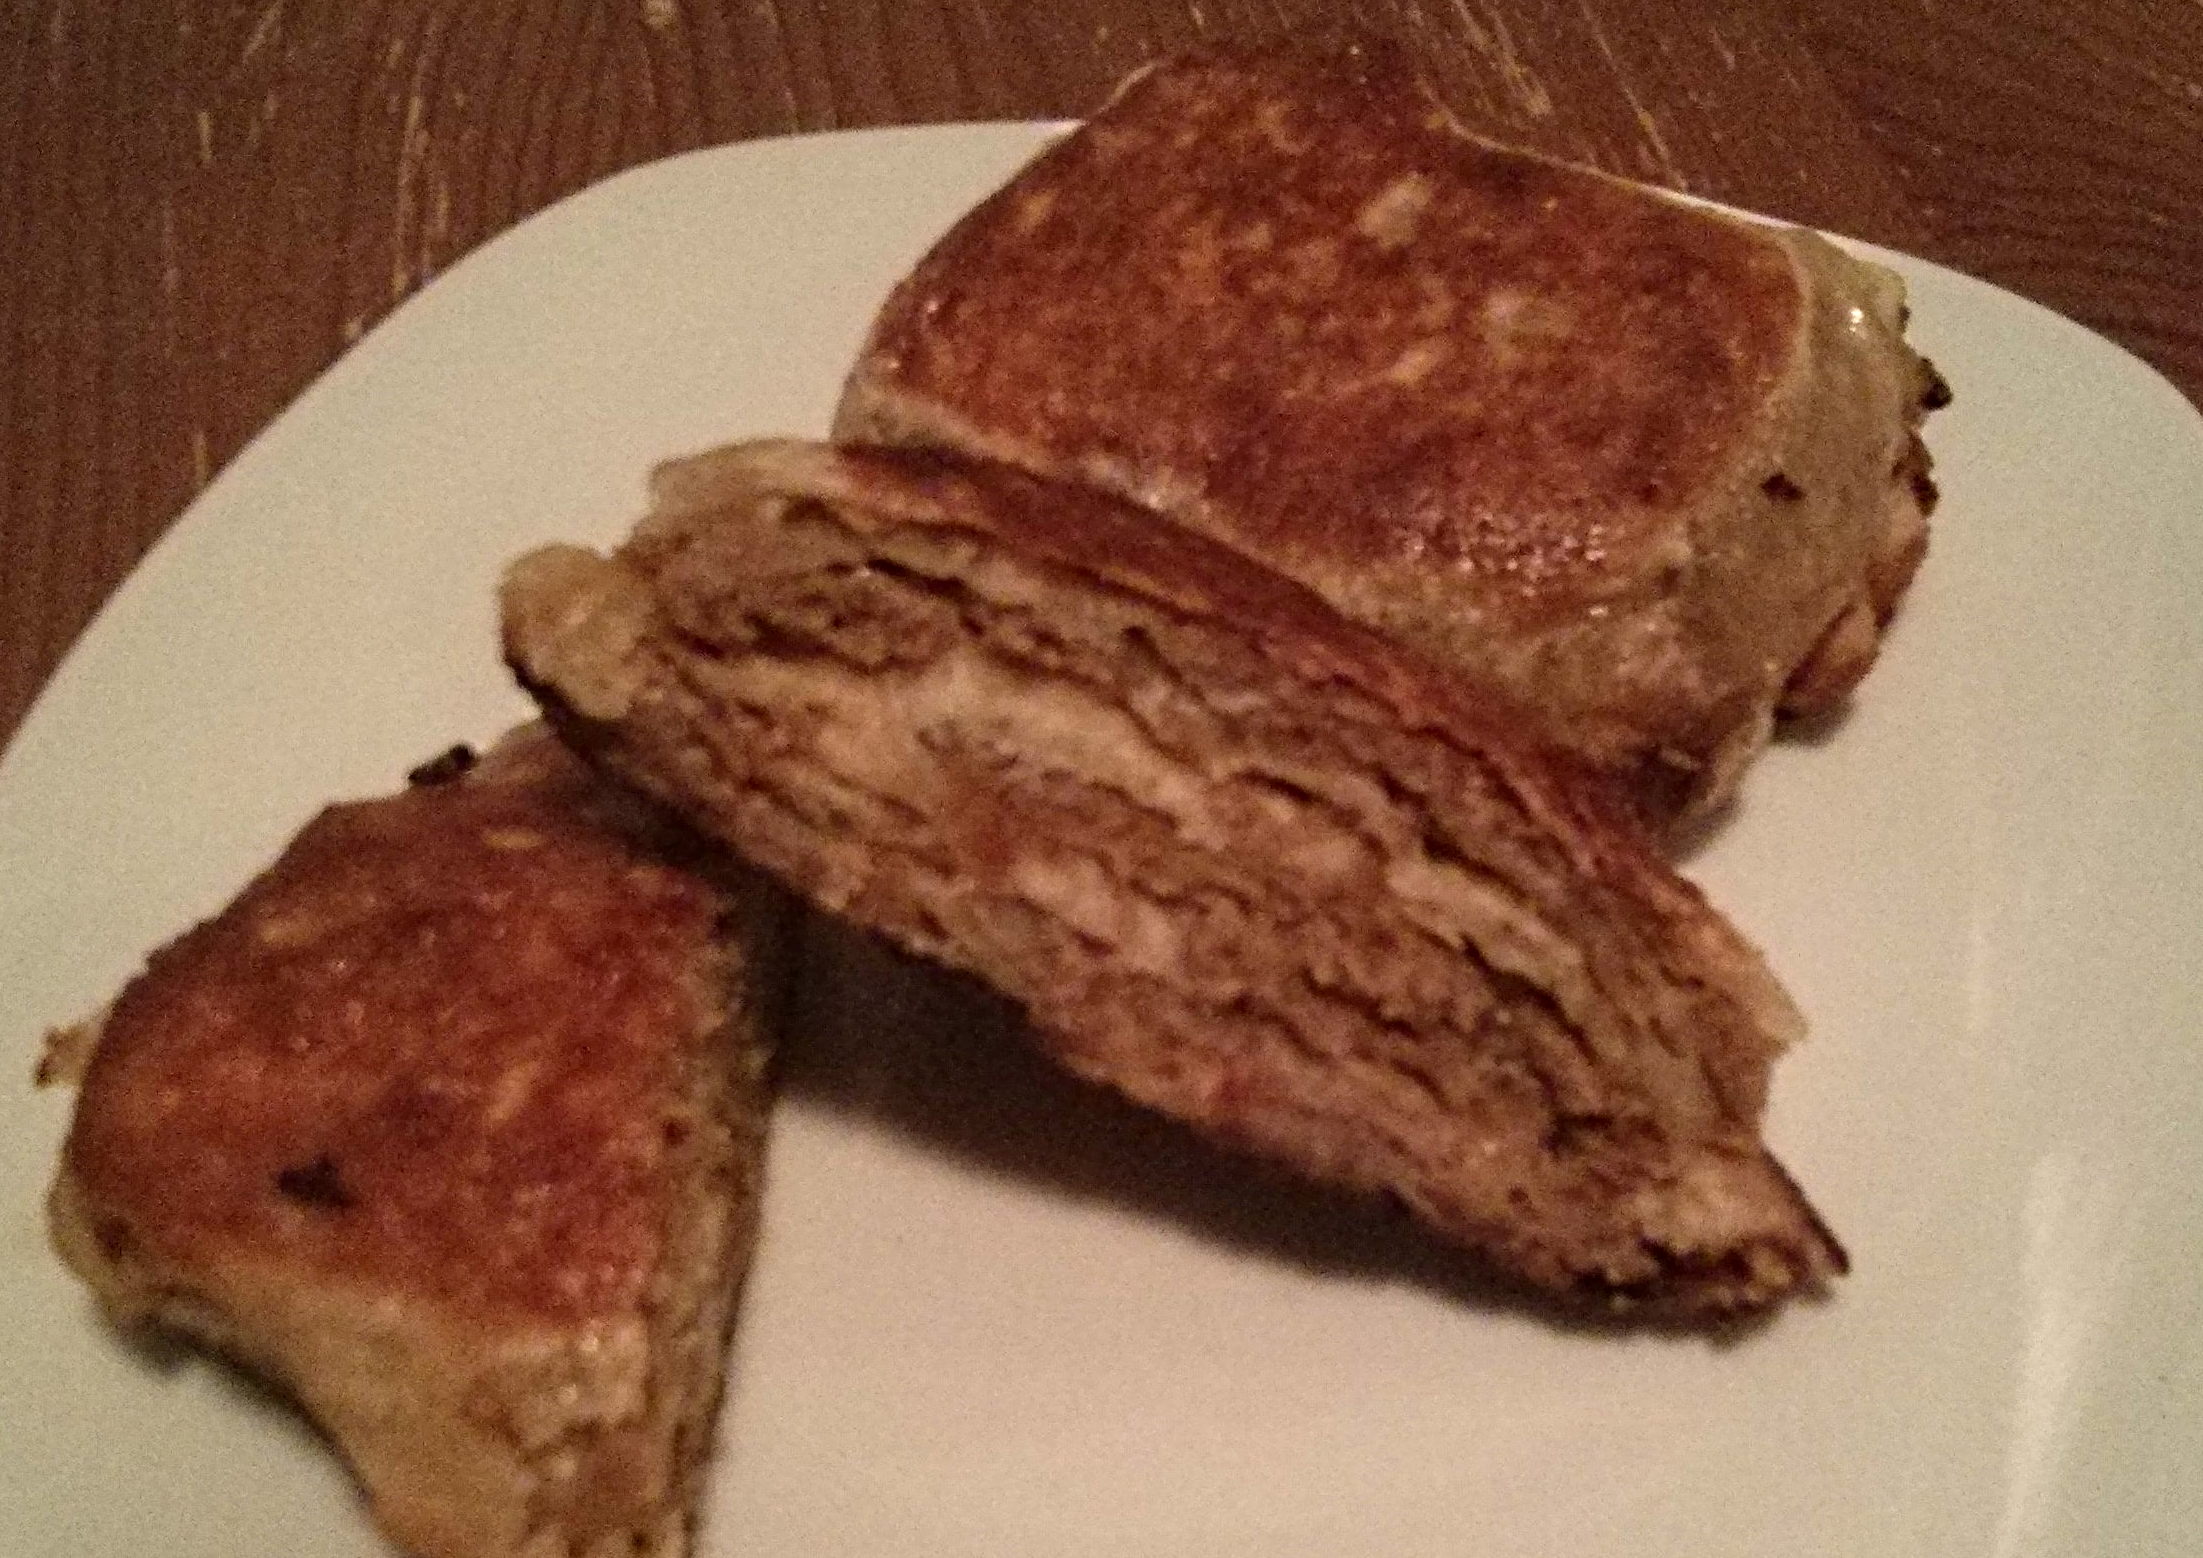
\includegraphics[width=\paperwidth,height=\paperheight]{./bilder/curry-hack-pancakes_ratio.jpg}};

\begin{recipe}[]{Curry-Hack-Pancakes} %Quelle
	\timerecipe[Minuten]{ca. 30+10+30} %mit [EINHEIT]
	\personcount{3} % mit[ART]
	\ingredient{100g Mehl} % ggf. \nicefrac{1}{2}
	\ingredient{1,5 TL Tockenhefe}
	\ingredient{0,75 EL Zucker}
	\ingredient{2 Prisen Salz}
	\ingredient{0,75 EL Sesamöl}
	\ingredient{65ml warmes Wasser}
	\ingredient{1 Ziebel}
	\ingredient{200g Hackfleisch}
	\ingredient{1,5 EL Sojasauce}
	\ingredient{1 EL Worcestersauce}
	\ingredient{1 EL Austernsauce}
	\ingredient{0,25 TL Pfeffer}
	\ingredient{2 TL Currypulver}
	\ingredient{2 EL Speisestärke}

\step
\textbf{100g Mehl}, \textbf{1,5 TL Tockenhefe}, \textbf{0,75 EL Zucker}, \textbf{1 Prisen Salz}, \textbf{0,75 EL Sesamöl} und \textbf{65ml warmes Wasser} zu einem Teig kneten und 30 Minuten ruhen lassen.

\step
\textbf{1 Zwiebel} klein würfeln und in der Pfanne anschwitzen, etwas abkühlen lassen und mit \textbf{200g Hackfleisch}, \textbf{1,5 EL Sojasauce}, \textbf{1 EL Worcestersauce}, \textbf{1 EL Austernsauce}, \textbf{0,25 TL Pfeffer}, \textbf{2 TL Currypulver} und \textbf{2 EL Speisestärke} für die Füllung mischen.

\step
Den Teig in 3 Stücke teilen, jeweils dünn und nahezu rechteckig ausrollen, jeweils gleichmäßig mit Füllung bestreichen. Zum Falten der Taschen das Rechteck zweimal pro langer Seite bis 1/3 der Breite einschneiden. Es sollten neun "gedachte" Quadrate entstehen.

\step
Jetzt jeweils an den Seiten die oberen und unteren Quadrate in die Mitte einklappen. Dann diese Quatrate ganz in die Mitte falten und mit den Klappen von oben und unten einklappen, so dass ein Paket entsteht. Ebenso mit den anderen Teigen verfahren.

\step
Ca. 8 - 10 Minuten mit geschlossenem Deckel auf beiden Seiten goldbraun braten (ca. 4 - 5 Minuten auf jeder Seite).

%\tippbox{\textbf{Tipp:} ...} % Tipp in extra Rahmen
\end{recipe}
\newpage
\tikz[remember picture,overlay] \node[opacity=1,inner sep=0pt] at (current page.center){\includegraphics[width=\paperwidth,height=\paperheight]{./bilder/gebackene_forelle_ratio.jpg}};

\begin{recipe}[]{Gebackene Forelle} %Quelle
	\timerecipe[Minuten]{ca. 15+40 } %mit [EINHEIT]
	\personcount[Forelle]{1} % mit[ART]
	\ingredient{1 frische Forelle} % ggf. \nicefrac{1}{2}
	\ingredient{2 Zwiebeln}
	\ingredient{1 Bund Petersilie}
	\ingredient{0,25l Weißwein}
	\ingredient{0,25l Brühe}
	\ingredient{Zitronensaft}
	\ingredient{Semelbrösel}
	\ingredient{75g geschmolzene Butter}
	\ingredient{Salz}
	\ingredient{Pfeffer}

\step
\textbf{2 Zwiebeln} in Ringe schneiden und \textbf{1 Bund Petersilie} waschen und zupfen. \textbf{Forelle} waschen und mit Zwiebeln und Petersilie füllen. 

\step
Forelle in Auflaufform legen und mit \textbf{0,25l Weißwein}, \textbf{0,25l Brühe} und \textbf{Zitronensaft} übergießen. \textbf{Salzen} und \textbf{pfeffern} und mit \textbf{Semelbröseln} bedecken. \textbf{75g geschmolzene Butter} darüber träufeln.

\step
35-40 Minuten bei 200-220°C auf der 2. untersten Schiene backen.

\tippbox{\textbf{Tipp:} Es kann auch weiteres Gemüse, wie beispielweise Tomaten mitgegart werden.} % Tipp in extra Rahmen
\end{recipe}
\newpage
\tikz[remember picture,overlay] \node[opacity=1,inner sep=0pt] at (current page.center){\includegraphics[width=\paperwidth,height=\paperheight]{./bilder/kuerbis_flammkuchen_ratio.jpg}};

\begin{recipe}[]{Kürbis-Flammkuchen} %Quelle
	\timerecipe[Minuten]{ca. 10+30} %mit [EINHEIT]
	\personcount[Blech]{1} % mit[ART]
	\ingredient{350g Mehl} % ggf. \nicefrac{1}{2}
	\ingredient{0,5 TL Zucker}
	\ingredient{0,5 TL Salz}
	\ingredient{3 EL Olivenöl}
	\ingredient{175ml Wasser}
	\ingredient{250g Hokkaidokürbis}
	\ingredient{1 große Zwiebel}
	\ingredient{100g Speckwürfel}
	\ingredient{1 Birne}
	\ingredient{200g Schmand}
	\ingredient{1 Feta}


\step
\textbf{350g Mehl}, \textbf{0,5 TL Zucker}, \textbf{0,5 TL Salz}, \textbf{3 EL Olivenöl} und \textbf{175ml Wasser} zu einem Teig kneten.

\step
\textbf{1 Zwiebel} in Ringe schneiden, \textbf{250g Hokkaidokürbis} in 0,5cm dicke Scheiben schneiden, \textbf{1 Birne} in Spalten schneiden und \textbf{1 Feta} in Würfel schneiden.

\step
Teig ausrollen, mit \textbf{200g Schmand} bestreichen, mit \textbf{Salz} und \textbf{Pfeffer} würzen und mit \textbf{100g Speckwürfeln}, den Kürbisschnitzen, den Birnenspalten, den Fetawürfeln und den Zwiebelringen belegen.

\step 
Ca. 25 Minuten bei 250°C (230°C Umluft) backen.

%\tippbox{\textbf{Tipp:} ...} % Tipp in extra Rahmen
\end{recipe}
\newpage

\begin{recipe}[]{Zwiebelkuchen} %Quelle http://www.chefkoch.de/rezepte/drucken/1716851280413039/2309481a/1/Einfacher-Zwiebelkuchen.html
	\timerecipe[Minuten]{ca. 5+30+5+30} %mit [EINHEIT]
	\personcount[Blech]{1} % mit[ART]
	\ingredient{450g Mehl} % ggf. \nicefrac{1}{2}
	\ingredient{50g Butter}
	\ingredient{1 Pk Trockenhefe}
	\ingredient{800g Zwiebeln}
	\ingredient{200g Speck}
	\ingredient{3 Eier}
	\ingredient{200ml Sahne}
	\ingredient{250g Käse}


\step
\textbf{450g Mehl}, \textbf{1 Pk Trockenhefe}, \textbf{1 TL Zucker}, \textbf{1 TL Salz}, \textbf{220ml Wasser} und \textbf{50g weiche Butter} zu einem Teig kneten.

\step
Den Teig 30 Minuten ruhen lassen. 

\step
\textbf{800g Zwiebeln} in Streifen schneiden und mit \textbf{200g Speck} anbraten.

\step
\textbf{3 Eier} mit \textbf{200ml Sahne} mischen und mit Salz, Muskat und Pfeffer würzen. Mit den Zwiebeln mischen und auf dem Teig verteilen und mit \textbf{250g Käse} bestreuen.

\step 
Ca. 30 Minuten bei 200°C (180°C Umluft) backen.

\tippbox{\textbf{Tipp:} Umbedingt mit Federweißer servieren. } % Tipp in extra Rahmen
\end{recipe}

\newpage
{\vspace*{4cm}\section{zu Nudeln}}
\begin{recipe}[]{Gulasch nach Art des Hauses Klenk}
	\timerecipe[Minuten]{ca. ?? + 120} %mit [EINHEIT]
	\personcount{5} % mit[ART]
	\ingredient{750g Rindergulasch} % ggf. \nicefrac{1}{2}
	\ingredient{3 große Zwiebeln}
	\ingredient{2 Knoblauchzehen}
	\ingredient{3 Gemüsepaprika}
	\ingredient{etwas Tomatenmark}
	\ingredient{1 Becher Sahne}
	\ingredient{(1 Glas Rotwein)}
	
\step
\textbf{750g Rindergulasch} in Öl portionsweise scharf anbraten.

\step
Die in grobe Ringe geschnittenen \textbf{3 große Zwiebeln} und die kleingehackten \textbf{2 Knoblauchzehen} dazugeben und kurz anbraten.

\step
Die \textbf{3 Paprika} in Streifen geschnitten dazugeben und nach kurzem anbraten mit \textbf{Gemüsebrühe} und evt. \textbf{einem Glas Rotwein} aufgießen.

\step
Pfeffer und Salz dazugeben und bei geringer Hitze zugedeckt schmurgeln lassen. Immer mal kontrollieren, ob genug Flüssigkeit da ist.

\step
Nach ca. 1,5-2 Stunden \textbf{einen Becher Sahne} dazugeben und mit Paprikapulver abschmecken. Tabasco macht das Ganze schärfer.





%\tippbox{{Tipp:} ...} % Tipp in extra Rahmen
\end{recipe}
\begin{recipe}[]{Gulasch für Josi und Max} %Max
	\timerecipe[Minuten]{ca. ?? + 120} %mit [EINHEIT]
	\personcount{2} % mit[ART]
	\ingredient{500g Rindergulasch} % ggf. \nicefrac{1}{2}
	\ingredient{2 große Zwiebeln}
	\ingredient{2 Knoblauchzehen}
	\ingredient{2 Gemüsepaprika}
	\ingredient{etwas Tomatenmark}
	\ingredient{1 Becher Sahne}
	\ingredient{(1 Glas Rotwein)}
	
\step
\textbf{500g Rindergulasch} in Öl portionsweise scharf anbraten.

\step
Die in grobe Ringe geschnittenen \textbf{2 große Zwiebeln} und die kleingehackten \textbf{2 Knoblauchzehen} dazugeben und kurz anbraten.

\step
Die \textbf{2 Paprika} in Streifen geschnitten dazugeben und nach kurzem anbraten mit \textbf{Gemüsebrühe} und evt. \textbf{einem Glas Rotwein} aufgießen.

\step
Pfeffer und Salz dazugeben und bei geringer Hitze zugedeckt schmurgeln lassen. Immer mal kontrollieren, ob genug Flüssigkeit da ist.

\step
Nach ca. 1,5-2 Stunden \textbf{einen Becher Sahne} dazugeben und mit Paprikapulver abschmecken. Tabasco macht das Ganze schärfer.


%\tippbox{{\bf Tipp:} ...} % Tipp in extra Rahmen
\end{recipe}
\begin{recipe}[]{Hackfleischsoße} %MUTTI Dez
	\timerecipe[Minuten]{ca. } %mit [EINHEIT]
	\personcount[Klenks]{5} % mit[ART]
	\ingredient{500g Hackfleisch gemischt} % ggf. \nicefrac{1}{2}
	\ingredient{2 Zwiebeln}
	\ingredient{2 Knoblauchzehen}
	\ingredient{3 Karotten}
	\ingredient{1 Dose Tomaten}
	\ingredient{1 Dose passierte Tomaten}

\step
\textbf{500g gemischtes Hackfleisch} mit Öl in der Pfanne anbraten, die gewürfelte \textbf{2 Zwiebel} und die klein geschnittenen \textbf{2 Knoblauchzehen} sowie die gewürfelten \textbf{3 Karotten} dazugeben und andünsten, bis die Zwiebeln glasig sind.

\step
Die \textbf{Dosentomaten}, die \textbf{passierten Tomaten} und \textbf{2-3 EL Tomatenmark} dazugeben und mit der gleichen Menge \textbf{Wasser} auffüllen. Mit \textbf{Gemüsebrühe}, \textbf{Salz}, \textbf{Pfeffer}, \textbf{1 EL Zucker} und \textbf{Herbes de Provence} würzen.

\step
Solange köcheln, bis die Karotten weich sind. Wenn die Soße zu dickflüssig ist, mit Wasser verdünnen.




%\tippbox{{\bf Tipp:} ...} % Tipp in extra Rahmen
\end{recipe}
\begin{recipe}[]{Saltimbocca a la romana} % MUTTI Feb 14
	\timerecipe[Minuten]{ca. } %mit [EINHEIT]
	\personcount[Personen]{4} % mit[ART]
	\ingredient{8 kleine Kalbsschnitzel} % ggf. \nicefrac{1}{2}
	\ingredient{4 luftgetrockneter Schinken}
	\ingredient{8-16 Salbeiblättchen}
	\ingredient{50ml trockener Weißwein}

\step
Die \textbf{8 Kalbsschnitzel} mit dem Handballen etwas flach drücken.

\step
Jedes Schnitzel mit einem \textbf{halben Schinkenstück} und \textbf{1-2 Salbeiblättchen} belegen und mit Zahnstocher fest stecken. 

\step
Die Schnitzel auf der unbelegten Seite \textbf{salzen} und \textbf{pfeffern}. 

\step
Den Backofen auf 70 °C vorheizen. 

\step
\textbf{2 Eßl. Butter} in einer Pfanne zerlassen. Die Hälfte der Schnitzel mit der Salbeiseite nach unten hineinlegen und bei mittlerer Hitze 2 min braten. Wenden und nochmals 1 min braten, dann auf einem Teller im Ofen warm stellen.

\step
Die restliche Schnitzel wie beschrieben braten und in den Ofen geben.

\step
\textbf{50ml Wein} in die Pfanne gießen und den Bratensatz damit loskochen. Sauce über die Schnitzel gießen rasch servieren. Dazu schmecken Weißbrot oder Nudeln.

%\tippbox{{\bf Tipp:} ...} % Tipp in extra Rahmen
\end{recipe}
\begin{recipe}[]{Zucchinisoße} %MAX
	\timerecipe[Minuten]{ca. } %mit [EINHEIT]
	\personcount[Personen]{5} % mit[ART]
	\ingredient{1 kg Zucchini} % ggf. \nicefrac{1}{2}
	\ingredient{3 Zwiebeln}
	\ingredient{2 Knoblauchzehen}
	\ingredient{2 Becher Sahne}
	\ingredient{Gemüsebrühe}
	\ingredient{geriebener Käse}


\step
\textbf{1kg Zucchini} waschen und mit einer groben Reibe zerkleinern.

\step
Die gewürfelte \textbf{3 Zwiebel} und die klein geschnittenen \textbf{2 Knoblauchzehen} in Öl andünsten.

\step
Nun die Zucchini zugeben und mit \textbf{Gemüsebrühe} ablöschen.

\step
Die \textbf{2 Becher Sahne} untermischen und mit Salz und Pfeffer abschmecken.

%\tippbox{{\bf Tipp:} ...} % Tipp in extra Rahmen
\end{recipe}

\newpage
{\vspace*{4cm}\section{unsortiert}}
\begin{recipe}[]{Königsberger Klopse} % MUTTI Nov
	\timerecipe[Minuten]{ca. 60 } %mit [EINHEIT]
	\personcount[Personen]{4} % mit[ART]
	\ingredient{500g Hackfleisch gemischt} % ggf. \nicefrac{1}{2}
	\ingredient{2 Scheiben Weißbrot}
	\ingredient{2 Zwiebel}
	\ingredient{2 Nelken}
	\ingredient{3 EL Petersilie}
	\ingredient{3 EL Sahne}
	\ingredient{1 Lorbeerblatt}
	\ingredient{3 EL Butter}
	\ingredient{2 EL Mehl}
	\ingredient{2 EL Zitronensaft}
	\ingredient{2 EL Kapern}

\step
Aus den \textbf{500g Hackfleisch}, den \textbf{2 Scheiben Weißbrot},
\textbf{einer klein gehackten Zwiebel} und \textbf{3 EL Petersilie} 
einen Hackfleischteig herstellen und Klopse formen.

\step
\textbf{1 Liter Salzwasser} zum Kochen bringen und Temperatur runter schalten. 

\step
Das \textbf{Lorbeerblatt} und die mit den \textbf{2 Nelken} gespickte \textbf{Zwiebel} zugeben.
Die Klopse in das nicht mehr kochende Wasser geben und 15-20 min gar ziehen lassen.

\step
\textbf{2 EL Mehl} in \textbf{2EL zerlassener Butter} anschwitzen, bis es goldgelb ist. Dann den Topf von der Herdplatte nehmen und die Flüssigkeit nach und nach einrühren (Schneebesen).

\step
Die Soße 10 min kochen lassen uns dann \textbf{2 EL Kapern}, \textbf{2 EL Zitronensaft} und \textbf{3 EL Sahne} hinzugeben. Klopse hineigeben und abschmecken.

%\tippbox{{\bf Tipp:} ...} % Tipp in extra Rahmen
\end{recipe}
\begin{recipe}[]{Frikadellen} %http://www.chefkoch.de/rezepte/819141186405890/Omas-beste-Frikadellen.html
	\timerecipe[Minuten]{ca. ?? } %mit [EINHEIT]
	\personcount{4} % mit[ART]
	\ingredient{500g Hackfleisch (gemischt)} % ggf. \nicefrac{1}{2}
	\ingredient{1 Zwiebel}
	\ingredient{1 Brötchen}
	\ingredient{1 Ei}
	\ingredient{1 TL Senf}
	\ingredient{Semmelbrösel}

\step
\textbf{Ein Brötchen} in Wasser einweichen. Die \textbf{Zwiebel} schälen und in feine Würfel schneiden und kurz anbraten.

\step
Das \textbf{Ei}, die \textbf{Zwiebel}, \textbf{1 TL Salz}, \textbf{1 TL Senf}, \textbf{1 TL Paprikapulver} und \textbf{viel Pfeffer} zum \textbf{Hackfleisch} geben und sehr gut mit den Händen vermengen. 

\step
Die Brötchenmasse sehr gut ausdrücken, zur Hackmasse geben und wieder gut vermengen.

\step
Jetzt gleichmäßige Bällchen formen und auf einer be\textbf{mehl}ten Arbeitsfläche flachdrücken und anschließend in \textbf{Semmelbrösel} wenden. 

\step
Eine Pfanne mit \textbf{Butter} stark erhitzen und die Frikadellen einlegen, kurz auf beiden Seiten scharf anbraten und dann ca. 15 - 20 Minuten (1 - 2mal vorsichtig wenden) auf mittlerer/schwacher Hitze fertig braten.

%\tippbox{{\bf Tipp:} ...} % Tipp in extra Rahmen
\end{recipe}
\begin{recipe}[]{Geschmorte weiße Bohnen} % MUTTI Feb 14
	\timerecipe[Minuten]{ca. } %mit [EINHEIT]
	\personcount{} % mit[ART]
	\ingredient{200g kleine, weiße Bohnen (Cannellini)} % ggf. \nicefrac{1}{2}
	\ingredient{2 Lorbeerblätter}
	\ingredient{1 getrockneter Peperoncino}
	\ingredient{1 Dose Tomaten}
	\ingredient{3 Knoblauchzehen}
	\ingredient{4 Zweige Salbei}


\step
Die \textbf{Bohnen} mit kaltem Wasser bedecken und über Nacht einweichen. 

\step
Am nächsten Tag abgießen und mit frischem Wasser in den Topf füllen.

\step
\textbf{2 Lorbeerblätter} und \textbf{2 Teel. Pfefferkörner} mit leicht angedrücktem \textbf{Peperoncino} dazugeben. 

\step
Die Bohnen zum Kochen bringen und bei schwacher Hitze zugedeckt ca. 1-1\nicefrac{1}{2} Stunden fast weich garen. Am besten zwischendurch mal probieren.

\step
\textbf{3 Koblauchzehen} schälen und kleinhacken, \textbf{Salbeiblätter} in feine Streifen schneiden und beides zusammen in \textbf{Olivenöl} anbraten. Die \textbf{Dose Tomaten} dazugeben und köcheln lassen. 

\step
Die Bohnen abgießen, Lorbeer, Pfeffer und Peperoncino entfernen und zu den Tomaten geben. 
Alles mit \textbf{Salz} und \textbf{Pfeffer} würzen und noch ca. \nicefrac{1}{2} Stunde köcheln, bis die Bohnen weich genug sind.

\tippbox{{\bf Tipp:} Passt als Beilage zu Fleisch mit Nudeln oder Kartoffeln oder Weißbrot.} % Tipp in extra Rahmen
\end{recipe}
\begin{recipe}[]{Putengulasch mit Sauerkraut} % Max
	\timerecipe[Minuten]{ca. 15} %mit [EINHEIT]
	\personcount{3} % mit[ART]
	\ingredient{1 Zwiebel} % ggf. \nicefrac{1}{2}
	\ingredient{450g gewürztes Putengulasch}
	\ingredient{500g Sauerkraut}
	\ingredient{4 El Schmand}

\step
\textbf{1 Zwiebel} hacken und glasig schmoren.  Die \textbf{450g Putengulasch} mit anbraten.

\step
\textbf{500g Sauerkraut} zugeben und mit Salz, Pfeffer, Zucker und Paprikapulver würzen. \textbf{125ml Gemüsebrühe} anrühren und das ganze weitere 15 Minuten schmoren lassen.

\step
\textbf{4 El Schmand} unterheben und erneut abschmecken.

\step
Mit Salzkartoffeln servieren.

%\tippbox{{Tipp:} ...} % Tipp in extra Rahmen
\end{recipe}

\newpage
{\vspace*{4cm}\section{Süßes}}
\begin{recipe}[]{Apfelstrudel} %MUTTI Nov
	\timerecipe[Minuten]{ca. } %mit [EINHEIT]
	\personcount[Blech]{1} % mit[ART]
	\ingredient{250g Mehl} % ggf. \nicefrac{1}{2}
	\ingredient{1 Ei}
	\ingredient{2kg Boskoop}
	\ingredient{1 Packung Rosinen}
	\ingredient{Vanillesoße}

\step
Die \textbf{250g Mehl} in eine Schüssel geben und \textbf{ein Ei}, \textbf{eine Prise Salz}, \textbf{etwas Wasser} und \textbf{ein TL Butter} in die Mitte geben. Alles zügig verkneten. Den Teig unter einem erwärmten Topf ca. \nicefrac{1}{2} Stunde ruhen lassen.

\step
In der Zwischenzeit die \textbf{2kg Boskoop} schälen und in Würfel schneiden.
Die \textbf{Rosinen} in warmem Wasser einweichen.

\step
\textbf{4 EL Semmelbrösel} in einem Topf mit \textbf{3 EL Butter} bräunen und unter die Äpfel mischen.

\step
Den Teig auf einem be\textbf{mehl}ten Küchenhandtuch sehr dünn ausrollen (so dass man die Zeitung durchlesen kann), und die Äpfel mit den Rosinen und dem \textbf{Zimt} und \textbf{Zucker} in der Mitte verteilen. Den Teig zuklappen, die Enden einschlagen und mit Hilfe des Küchenhandtuchs auf ein Backblech mit Backpapier legen.

\step
Mit etwas geschmolzener \textbf{Butter} bestreichen und bei 200°C ca. \nicefrac{1}{2} Stunde backen. Auf die Farbe achten!

\step
Aus dem Ofen nehmen und mit Puderzucker bestreuen und noch warm mit kalter Vanillesoße servieren.


%\tippbox{{\bf Tipp:} ...} % Tipp in extra Rahmen
\end{recipe}
\begin{recipe}[]{Appelränzjer} %MUTTI 1
	\timerecipe[Minuten]{ca. } %mit [EINHEIT]
	\personcount{} % mit[ART]
	\ingredient{500g Mehl} % ggf. \nicefrac{1}{2}
	\ingredient{4 Eier}
	\ingredient{200ml Milch}
	\ingredient{3 Boskoop}

\step
Die \textbf{500g Mehl}, \textbf{4 Eier}, \textbf{200ml Milch} mit \textbf{etwas Sprudelwasser}  mischen, bis ein nicht zu flüssiger Teig entsteht.

\step
Die \textbf{3 Äpfel} schälen, das Kerngehäuse entfernen und die Äpfel in Scheiben schneiden.

\step
Einen Teelöffel \textbf{Butter} in einer Pfanne schmelzen lassen und 3 kleine Pfannkuchen in der Pfanne verteilen, je eine Apfelscheibe darauf geben und umdrehen, wenn die Unterseite gut gebacken ist.


%\tippbox{{\bf Tipp:} ...} % Tipp in extra Rahmen
\end{recipe}
\begin{recipe}[]{Obstmichel} %MUTTI 1
	\timerecipe[Minuten]{ca. ?? + 40} %mit [EINHEIT]
	\personcount[Auflaufform]{1} % mit[ART]
	\ingredient{5 Brötchen} % ggf. \nicefrac{1}{2}
	\ingredient{\nicefrac{1}{2} L Milch}
	\ingredient{50g Zucker}
	\ingredient{3 Eier}
	\ingredient{1 EL Mehl}
	\ingredient{1 Glas Kirschen}
	\ingredient{60g Butter}


\step
\textbf{5 Brötchen} in Würfel schneiden und in \textbf{\nicefrac{1}{2} Liter Milch} einweichen (am besten schon morgens).

\step
Ofen auf 180°C Ober-Unterhitze vorheizen.

\step
\textbf{3 Eier} trennen und Eiweiß steif schlagen.

\step
\textbf{60g Butter}, \textbf{50g Zucker} und Eigelb schaumig schlagen, \textbf{1 EL Mehl} dazugeben und vermischen.

\step
Die eingeweichten Brötchen darunter mischen und dann den Eischnee unterheben.

\step
\textbf{1 Glas Kirschen} in eine gefettete Auflaufform geben, den Teig darauf verteilen und mit Butterflöckchen und Semmelbröseln bedecken.

\step
Bei ca. 180°C ca. 40 min backen.





%\tippbox{{\bf Tipp:} ...} % Tipp in extra Rahmen
\end{recipe}
\newpage
\tikz[remember picture,overlay] \node[opacity=1,inner sep=0pt] at (current page.center){\includegraphics[width=\paperwidth,height=\paperheight]{./bilder/quarkauflauf_ratio.jpg}};

\begin{recipe}[]{Quarkauflauf} %MUTTI 1
	\timerecipe[Minuten]{ca. 20 + 40} %mit [EINHEIT]
	\personcount[Auflaufform]{1} % mit[ART]
	\ingredient{3 Eier} % ggf. \nicefrac{1}{2}
	\ingredient{75g Butter}
	\ingredient{150g Zucker}
	\ingredient{500g Magerquark}
	\ingredient{40g Speisestärke}
	\ingredient{60g Gries}
	\ingredient{\nicefrac{1}{2}  Päckchen Backpulver}
	\ingredient{1 Glas Kirschen}

\step
Ofen auf 180°C Ober-Unterhitze vorheizen.

\step
\textbf{3 Eier} trennen und Eiweiß steif schlagen.

\step
Eigelb, \textbf{150g Zucker} und \textbf{75g Butter} schaumig schlagen.

\step
\textbf{500g Quark}, die \textbf{40g Speisestärke} und die \textbf{60g Gries} sowie das \textbf{halbe Päckchen Backpulver} untermischen.

\step
Den Eischnee unterheben und auf das \textbf{Glas Kirschen} in die gefettete Auflaufform geben.

\step
Mit \textbf{Butter}flöckchen und \textbf{Semmelbröseln} bestreuen.

\step
Bei 180°C ca. 40 min bei Ober-Unterhitze backen.

%\tippbox{{Tipp:} ...} % Tipp in extra Rahmen
\end{recipe}
\begin{recipe}[]{Topfenpalatschinken} %Josi
	\timerecipe[Minuten]{ca. 30 + 45} %mit [EINHEIT]
	\personcount{3} % mit[ART]
	\ingredient{150g 	Mehl} % ggf. \nicefrac{1}{2}
	\ingredient{4 Eier}
	\ingredient{425ml Milch}
	\ingredient{200g Quark}
	\ingredient{100g saure Sahne}
	\ingredient{50g Butter}
	\ingredient{80g Zucker}
	\ingredient{1 Bio Zitrone}
	\ingredient{3 EL Rosinen}

\step
Im Backofen auf 180°C Ober/Unterhitze vorheizen.

\step
Aus \textbf{2 Eiern}, \textbf{150g Mehl}, \textbf{1 Prise Salz} und \textbf{300ml Milch} einen Teig rühren.

\step
Aus dem Teig Pfannkuchen backen.

\step
Für die Füllung \textbf{2 Eier} trennen und das Eiweiße steif schlagen.

\step
\textbf{50g Butter}, \textbf{50g Zucker}, die \textbf{beiden Eigelbe}, \textbf{eine Prise Salz} und die \textbf{Schale der Zitrone} schaumig rühren. \textbf{200g Quark}, \textbf{100g saure Sahne} und \textbf{3 EL Rosinen} unterrühren.

\step
Jeweils einen Palatschinken mit etwas Quarkmasse bestreichen, aufrollen und in die gefettete Auflaufform schichten (möglichst nur einlagig).

\step
Für die Eiermilch \textbf{\nicefrac{1}{8} Milch}, \textbf{ein Ei} und \textbf{3 EL Zucker} verrühren und über die Palatschinken gießen.

\step
Im Backofen bei 180°C 40-45 Minuten auf der unteren Schiene backen.

\step
Vor dem Servieren mit Puderzucker bestäuben. 

%\tippbox{{Tipp:} ...} % Tipp in extra Rahmen
\end{recipe}

\newpage
{\vspace*{4cm}\section{Kuchen}}
\begin{recipe}[]{Donauwelle}
	\timerecipe[Minuten]{ca. 40 + 40} %mit [EINHEIT]
	\personcount[Blech]{1} % mit[ART]
	\ingredient{250g Margarine} % ggf. \nicefrac{1}{2}
	\ingredient{400g Zucker}
	\ingredient{350g Mehl}
	\ingredient{6 Eier}
	\ingredient{1 Pk. Backpulver}
	\ingredient{2 Esslöffel Kakaopulver(zum backen)}
	\ingredient{1 Glas Kirschen}
	\ingredient{1 Liter Milch}
	\ingredient{2 Pk. Vanillepuddingpulver}
	\ingredient{250g Butter}
	\ingredient{2 Pk. dunkle Kuvertüre}
	

\step
Backofen auf \textbf{180°C Ober-Unterhitze} vorheizen.

\step
\textbf{250g Margarine}, \textbf{250g Zucker}, \textbf{350g Mehl}, \textbf{1 Päckchen Backpulver} und \textbf{6 Eier} zu einem glatten Teig verrühren.

\step
Die Hälfte des Teiges auf ein mit Backpapier ausgelegtes Blech streichen. Zu der anderen Hälfte \textbf{2 Esslöffel Kakaopulver} mischen und auf den hellen Teig streichen. Das abgetropfte \textbf{Glas Kirschen} gleichmäßig auf dem Teig verteilen.

\step
Bei 180°C, Ober-Unterhitze ca. 30-40 min backen und den Kuchen danach abkühlen lassen.

\step
\textbf{800ml Milch} mit \textbf{250g Butter} und \textbf{150g Zucker} verrühren und zum Kochen bringen. Die mit den restlichen \textbf{200ml Milch} verrührten \textbf{2 Päckchen Puddingpulver} in die kochende Milch rühren und vom Herd nehmen.

\step
Die Creme auf dem Kuchen verteilen und abkühlen lassen.

\step
\textbf{2 Päckchen dunkle Kuvertüre} im Wasserbad schmelzen und auf dem Kuchen verteilen.




%\tippbox{{Tipp:} ...} % Tipp in extra Rahmen
\end{recipe}
\begin{recipe}[]{Käsekuchen nach Ester}
	\timerecipe[Minuten]{ca. } %mit [EINHEIT]
	\personcount{} % mit[ART]
	\ingredient{265g Butter} % ggf. \nicefrac{1}{2}
	\ingredient{315g Zucker}
	\ingredient{150g Mehl}
	\ingredient{7 Ei}
	\ingredient{1 TL Backpulver}
	\ingredient{2 Päckchen Vanillezucker}
	\ingredient{1 Päckchen Vanillepuddingpulver}
	\ingredient{750g Magerquark}

\step
Den Ofen auf 180°C Ober-Unterhitze vorheizen.

\step
\textbf{65g Butter}, \textbf{65g Zucker}, \textbf{150g Mehl}, \textbf{1 Ei}, \textbf{1 Teelöffel Backpulver} und \textbf{1 Päckchen Vanillezucker} zu einem Knetteig vermischen und \nicefrac{1}{2} Stunde in den Kühlschrank legen.

\step
\textbf{6 Eier} trennen und die Eiweiß zu steifem Schnee schlagen.

\step
Eigelb, \textbf{200g Butter}, \textbf{250g Zucker} und \textbf{1 Päckchen Vanillezucker} schaumig rühren, \textbf{750g Magerquark} und \textbf{1 Päckchen Vanillepuddingpulver} unterrühren. Den Eischnee vorsichtig mit dem Schneebesen unterheben.

\step
Den Teig auf dem Boden und am Rand einer eingefetteten Springform verteilen, die Quarkmasse darauf geben und bei 180°C Ober-Unterhitze, ca. 75 min backen. Zwischendurch die Farbe der Oberfläche kontrollieren. Falls der Kuchen zu dunkel wird mit Alufolie abdecken.

%\tippbox{{Tipp:} ...} % Tipp in extra Rahmen
\end{recipe}
\begin{recipe}[]{Apfel-Rahmkuchen} %MUTTI 1
	\timerecipe[Minuten]{ca. } %mit [EINHEIT]
	\personcount{} % mit[ART]
	\ingredient{200g Mehl} % ggf. \nicefrac{1}{2}
	\ingredient{3 Ei}
	\ingredient{150g Zucker}
	\ingredient{1 Päckchen Vanillezucker}
	\ingredient{100g Butter}
	\ingredient{1 Becher Schmand}
	\ingredient{20g Speisestärke}
	\ingredient{1kg Boskop}

\step
Aus \textbf{200g Mehl}, \textbf{1 Ei}, \textbf{50g Zucker}, \textbf{1 Päckchen Vanillezucker} und \textbf{100g Butter} einen Knetteig zubereiten und kalt stellen.

\step
Den Backofen auf 225°C Ober-Unterhitze vorheizen.

\step
Nach einer halben Stunde den Teig aus dem Kühlschrank nehmen, eine gefettete Springform damit auslegen und mit einer Gabel mehrere Male einstechen.

\step 
Bei 225°C Ober-Unterhitze ca. 10 min vorbacken.

\step
In der Zwischenzeit die \textbf{Äpfel} schälen, achteln und in grobe Würfel schneiden.

\step
Für den Guss \textbf{2 Eier} mit \textbf{100g Zucker} schaumig schlagen, \textbf{ein Becher Schmand} und \textbf{20g Speisestärke} dazugeben und unter Rühren kurz aufkochen.

\step
Die Äpfel auf den vorgebackenen Teig geben und dann den Guss darauf verteilen. Ungefähr 20 min fertigbacken.


%\tippbox{{\bf Tipp:} ...} % Tipp in extra Rahmen
\end{recipe}
\begin{recipe}[]{Biskuitrolle mit Himbeeren} %MUTTI Nov
	\timerecipe[Minuten]{ca. ?? + 15} %mit [EINHEIT]
	\personcount[Blech]{1} % mit[ART]
	\ingredient{4 Eier} % ggf. \nicefrac{1}{2}
	\ingredient{200g Zucker}
	\ingredient{2 Pk. Vanillezucker}
	\ingredient{80g Speisestärke}
	\ingredient{80g Mehl}
	\ingredient{1 TL Backpulver}
	\ingredient{2 Becher Sahne}
	\ingredient{500g Himbeeren}

\step
Backofen auf 225°C Ober-Unterhitze vorheizen und ggf. Himbeeren auftauen.

\step
\textbf{4 Eiweiß} steif schlagen.

\step
\textbf{4 Eigelb} mit \textbf{4 EL Wasser} und \textbf{200g Zucker} schaumig schlagen. Eiweiß oben drauf geben und mit \textbf{80g Mehl}, \textbf{80g Speisestärke} und \textbf{einem TL Backpulver} vorsichtig unterheben (Schneebesen).

\step
Den Teig sofort auf einem mit Backpapier ausgelegten Backblech verteilen und im Ofen ca. 13 Min. backen

\step
Danach auf ein mit Zucker bestreutes Küchenhandtuch kippen und locker zusammenrollen.

\step
\textbf{2 Becher Sahne} steif schlagen, \textbf{2 Päckchen Vanillezucker} und die \textbf{500g Himbeeren} unterheben und auf der abgekühlten, auseinander gerollten  Teigrolle verteilen. Zusammenrollen und mit \textbf{Puderzucker} bestreuen.

%\tippbox{{\bf Tipp:} ...} % Tipp in extra Rahmen
\end{recipe}
\begin{recipe}[]{Mandel-Zimtkuchen} % MUTTI Feb 14
	\timerecipe[Minuten]{ca. } %mit [EINHEIT]
	\personcount{} % mit[ART]
	\ingredient{65g Butter} % ggf. \nicefrac{1}{2}
	\ingredient{150g Mehl}
	\ingredient{4 Eier}
	\ingredient{125ml Sahne}
	\ingredient{125ml Milch}
	\ingredient{215g Zucker}
	\ingredient{200g gemahlene Mandeln}
	\ingredient{4 Zwieback (gerieben)}

\step
\textbf{65g Zucker}, \textbf{65g Butter}, \textbf{150g Mehl}, \textbf{1 Ei}, \textbf{1 Priese Salz} und \textbf{\nicefrac{1}{2} Teel. Backpulver} verkneten und 1 Stunde kalt stellen.

\step
Teig in einer Springfom ausrollen, mit einer Gabel mehrfach einstechen.

\step
Bei ca. 180 Grad auf mittlerer Schiene vorbacken, bis der Teig sich gebräunt hat.

\step
\textbf{3 Eier}, \textbf{125ml Sahne}, \textbf{125ml Milch}, \textbf{150g Zucker}, \textbf{1 Teel. Zimt} und \textbf{\nicefrac{1}{2} Teel. Backpulver} verrühren.

\step
\textbf{200g gemahlene Mandeln} und \textbf{4 Zwieback (gerieben)} unterheben und auf dem Bode verteilen.

\step
Den Kuchen ca. 45-50 Minuten fertig backen.

%\tippbox{{\bf Tipp:} ...} % Tipp in extra Rahmen
\end{recipe}
\begin{recipe}[]{Tante Evas Butterkuchen} %Josi Feb 14
	\timerecipe[Minuten]{ca. } %mit [EINHEIT]
	\personcount{} % mit[ART]
	\ingredient{250g Sahne} % ggf. \nicefrac{1}{2}
	\ingredient{500g Zucker}
	\ingredient{2 Pkt. Vanillezucker}
	\ingredient{4 Eier}
	\ingredient{500g Mehl}
	\ingredient{1 Pkt. Backpulver}
	\ingredient{\nicefrac{1}{2} Zitronen (Schale)}
	\ingredient{125g Butter}
	\ingredient{4 Eß. Milch}
	\ingredient{200g Mandeln} % halb gestiftet, halb Blättchen oder gehackt


\step
\textbf{250g Sahne} mit \textbf{250g Zucker}, \textbf{einem Pkt. Vanillezucker} und \textbf{4 Eiern} verrühren.

\step
Dazu \textbf{500g Mehl}, \textbf{1 Pkt. Backpulver}, \textbf{die Schale einer halben Zitronen} und \textbf{eine Priese Salz} unterrührern.

\step
Teig auf gefettetes Blech streichen und 10 Minuten bei 200 °c auf mittlerer Schiene backen.

\step
\textbf{250g Zucker}, \textbf{1 Pkt. Vanillezucker}, \textbf{125g Butter}, \textbf{4 Eß. Milch} und \textbf{200g Mandeln} zum Guß verrühren und auf den Teig krümmeln.

\step
Nochmals 10 Minuten auf der 2. Leiste backen.

%\tippbox{{Tipp:} ...} % Tipp in extra Rahmen
\end{recipe}
\begin{recipe}[]{Streuselkuchen} %Quelle: Pfadfinder
	\timerecipe[Minuten]{ca. 20 + 50} %mit [EINHEIT]
	\personcount[Blech]{1} % mit[ART]
	\ingredient{350g Butter} % ggf. \nicefrac{1}{2}
	\ingredient{350g Zucker}
	\ingredient{3 Eier}
	\ingredient{575g Mehl}
	\ingredient{1 Pck. Backpulver}
	\ingredient{1 Pck. Vanillinzucker}
	\ingredient{1 Glas Kirschen}
	\ingredient{4 Äpfel}

\step
Backofen auf 200°C (Umluft 180°C) vorheitzen.

\step
\textbf{200g Zucker} und \textbf{200g Butter} schaumig schlagen. Dann \textbf{3 Eier}, \textbf{1 Prise Salz}, \textbf{375g Mehl} und \textbf{1 Pck. Backpulver} unterrühren.

\step
Den Teig auf ein gefettetes oder mit Backpapier ausgelegtems Blech streichen.

\step
\textbf{1 Glas Kirschen} und \textbf{4 Äpfel} in Würfel geschnitten auf dem Teig verteilen.

\step
Für die Streusel \textbf{125g Butter} mit \textbf{150g Zucker}, \textbf{200g Mehl} und \textbf{1 Pck. Vanillinzucker} verrühren, daraus die Streusel kneten und auf dem Kuchen verteilen.

\step
Den Kuchen für \textbf{45-50 Minuten} backen.

%\tippbox{{Tipp:} ...} % Tipp in extra Rahmen
\end{recipe}

\newpage
\tikz[remember picture,overlay] \node[opacity=1,inner sep=0pt] at (current page.center){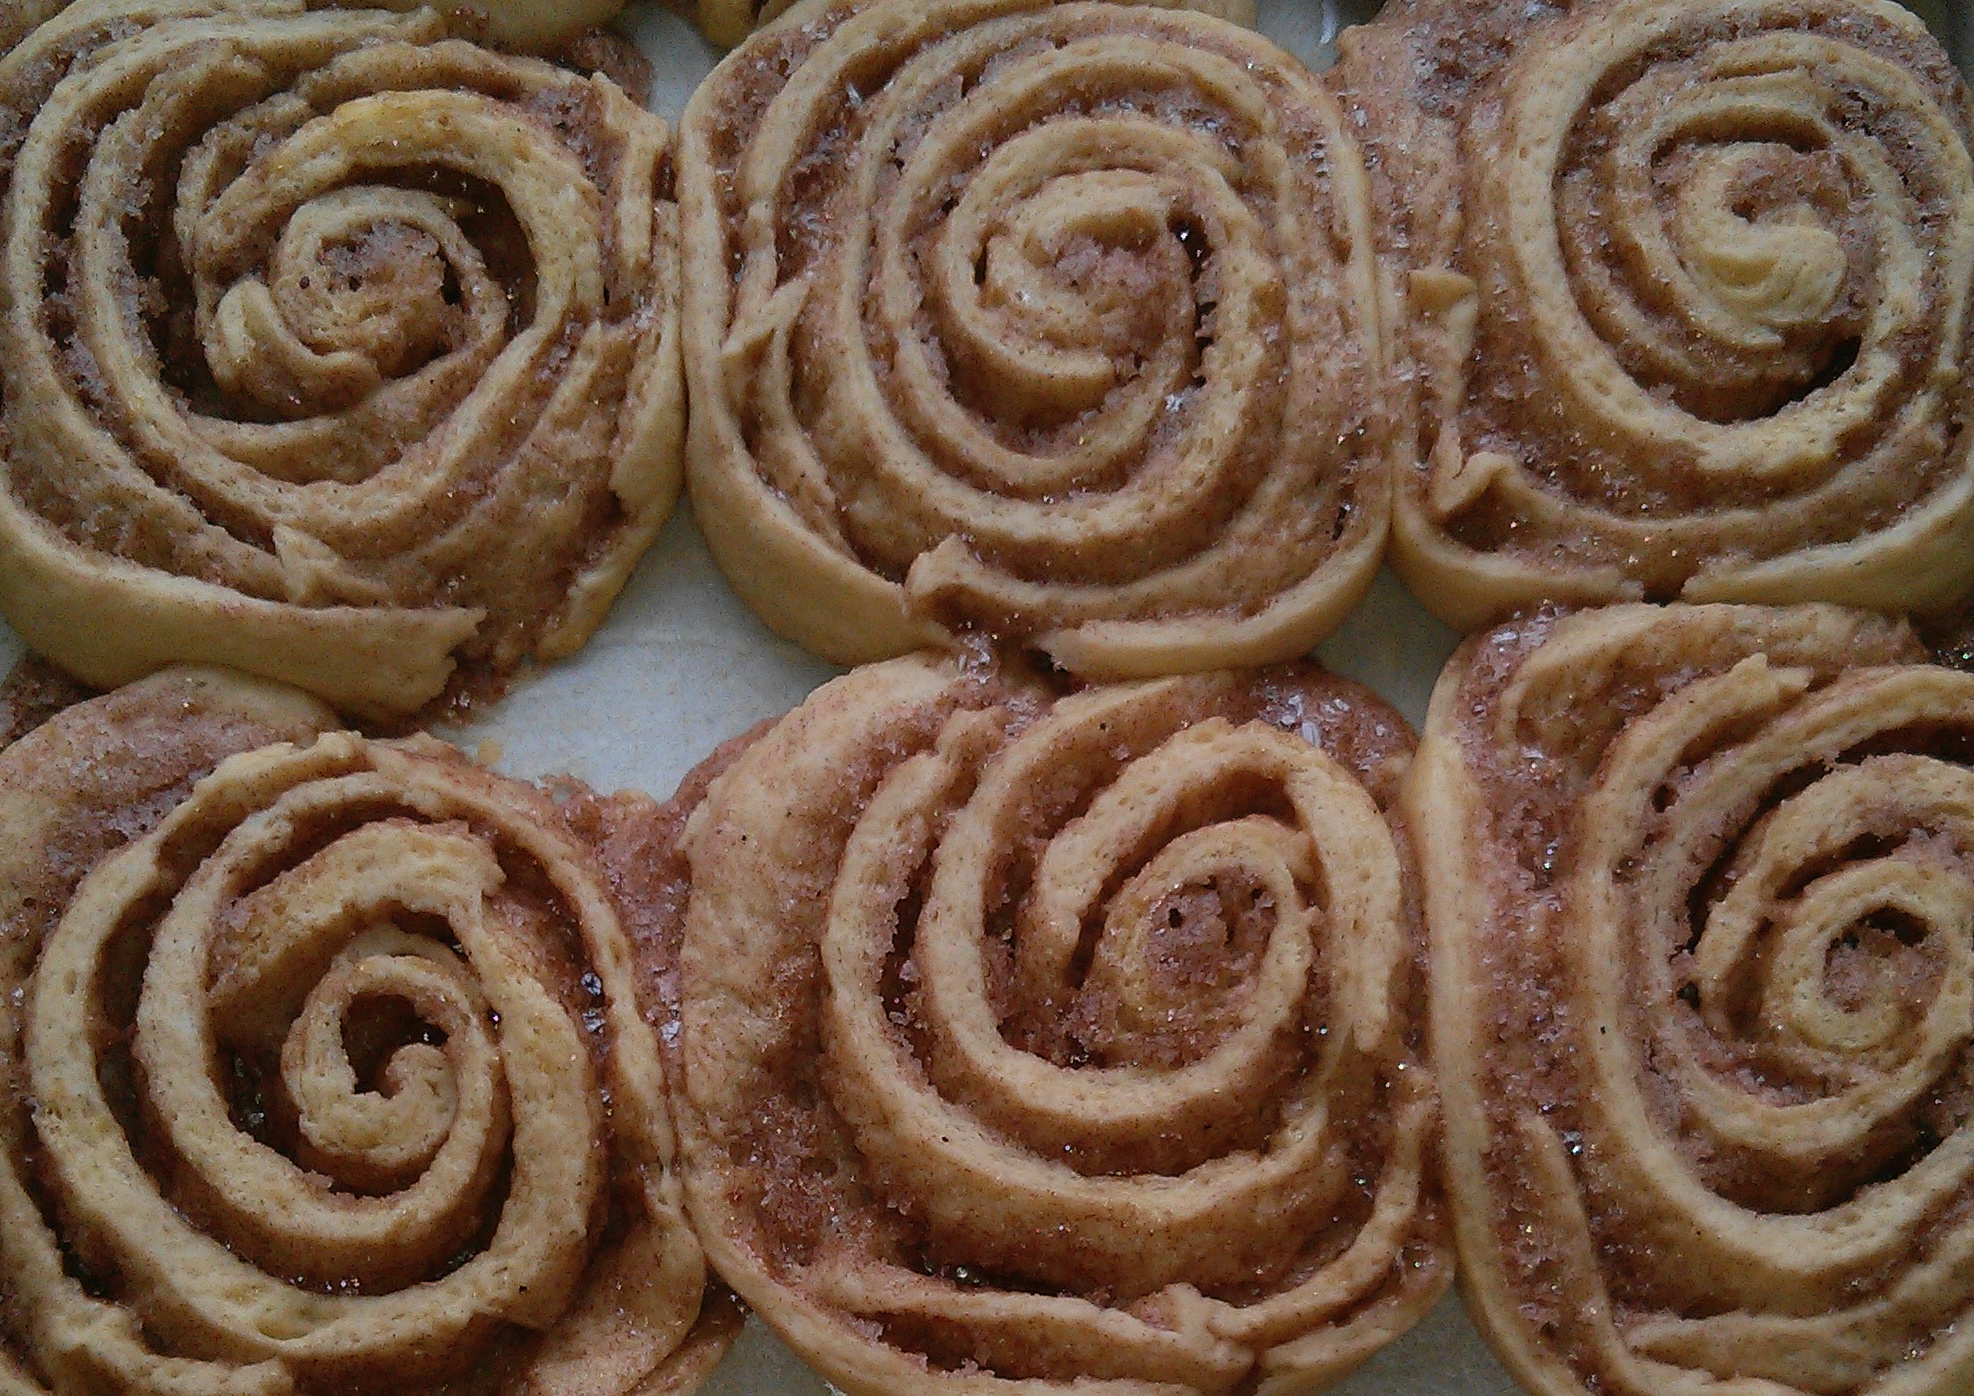
\includegraphics[width=\paperwidth,height=\paperheight]{./bilder/zimtschnecken_ratio.jpg}};


%\begin{center}
%  \makebox[\textwidth]{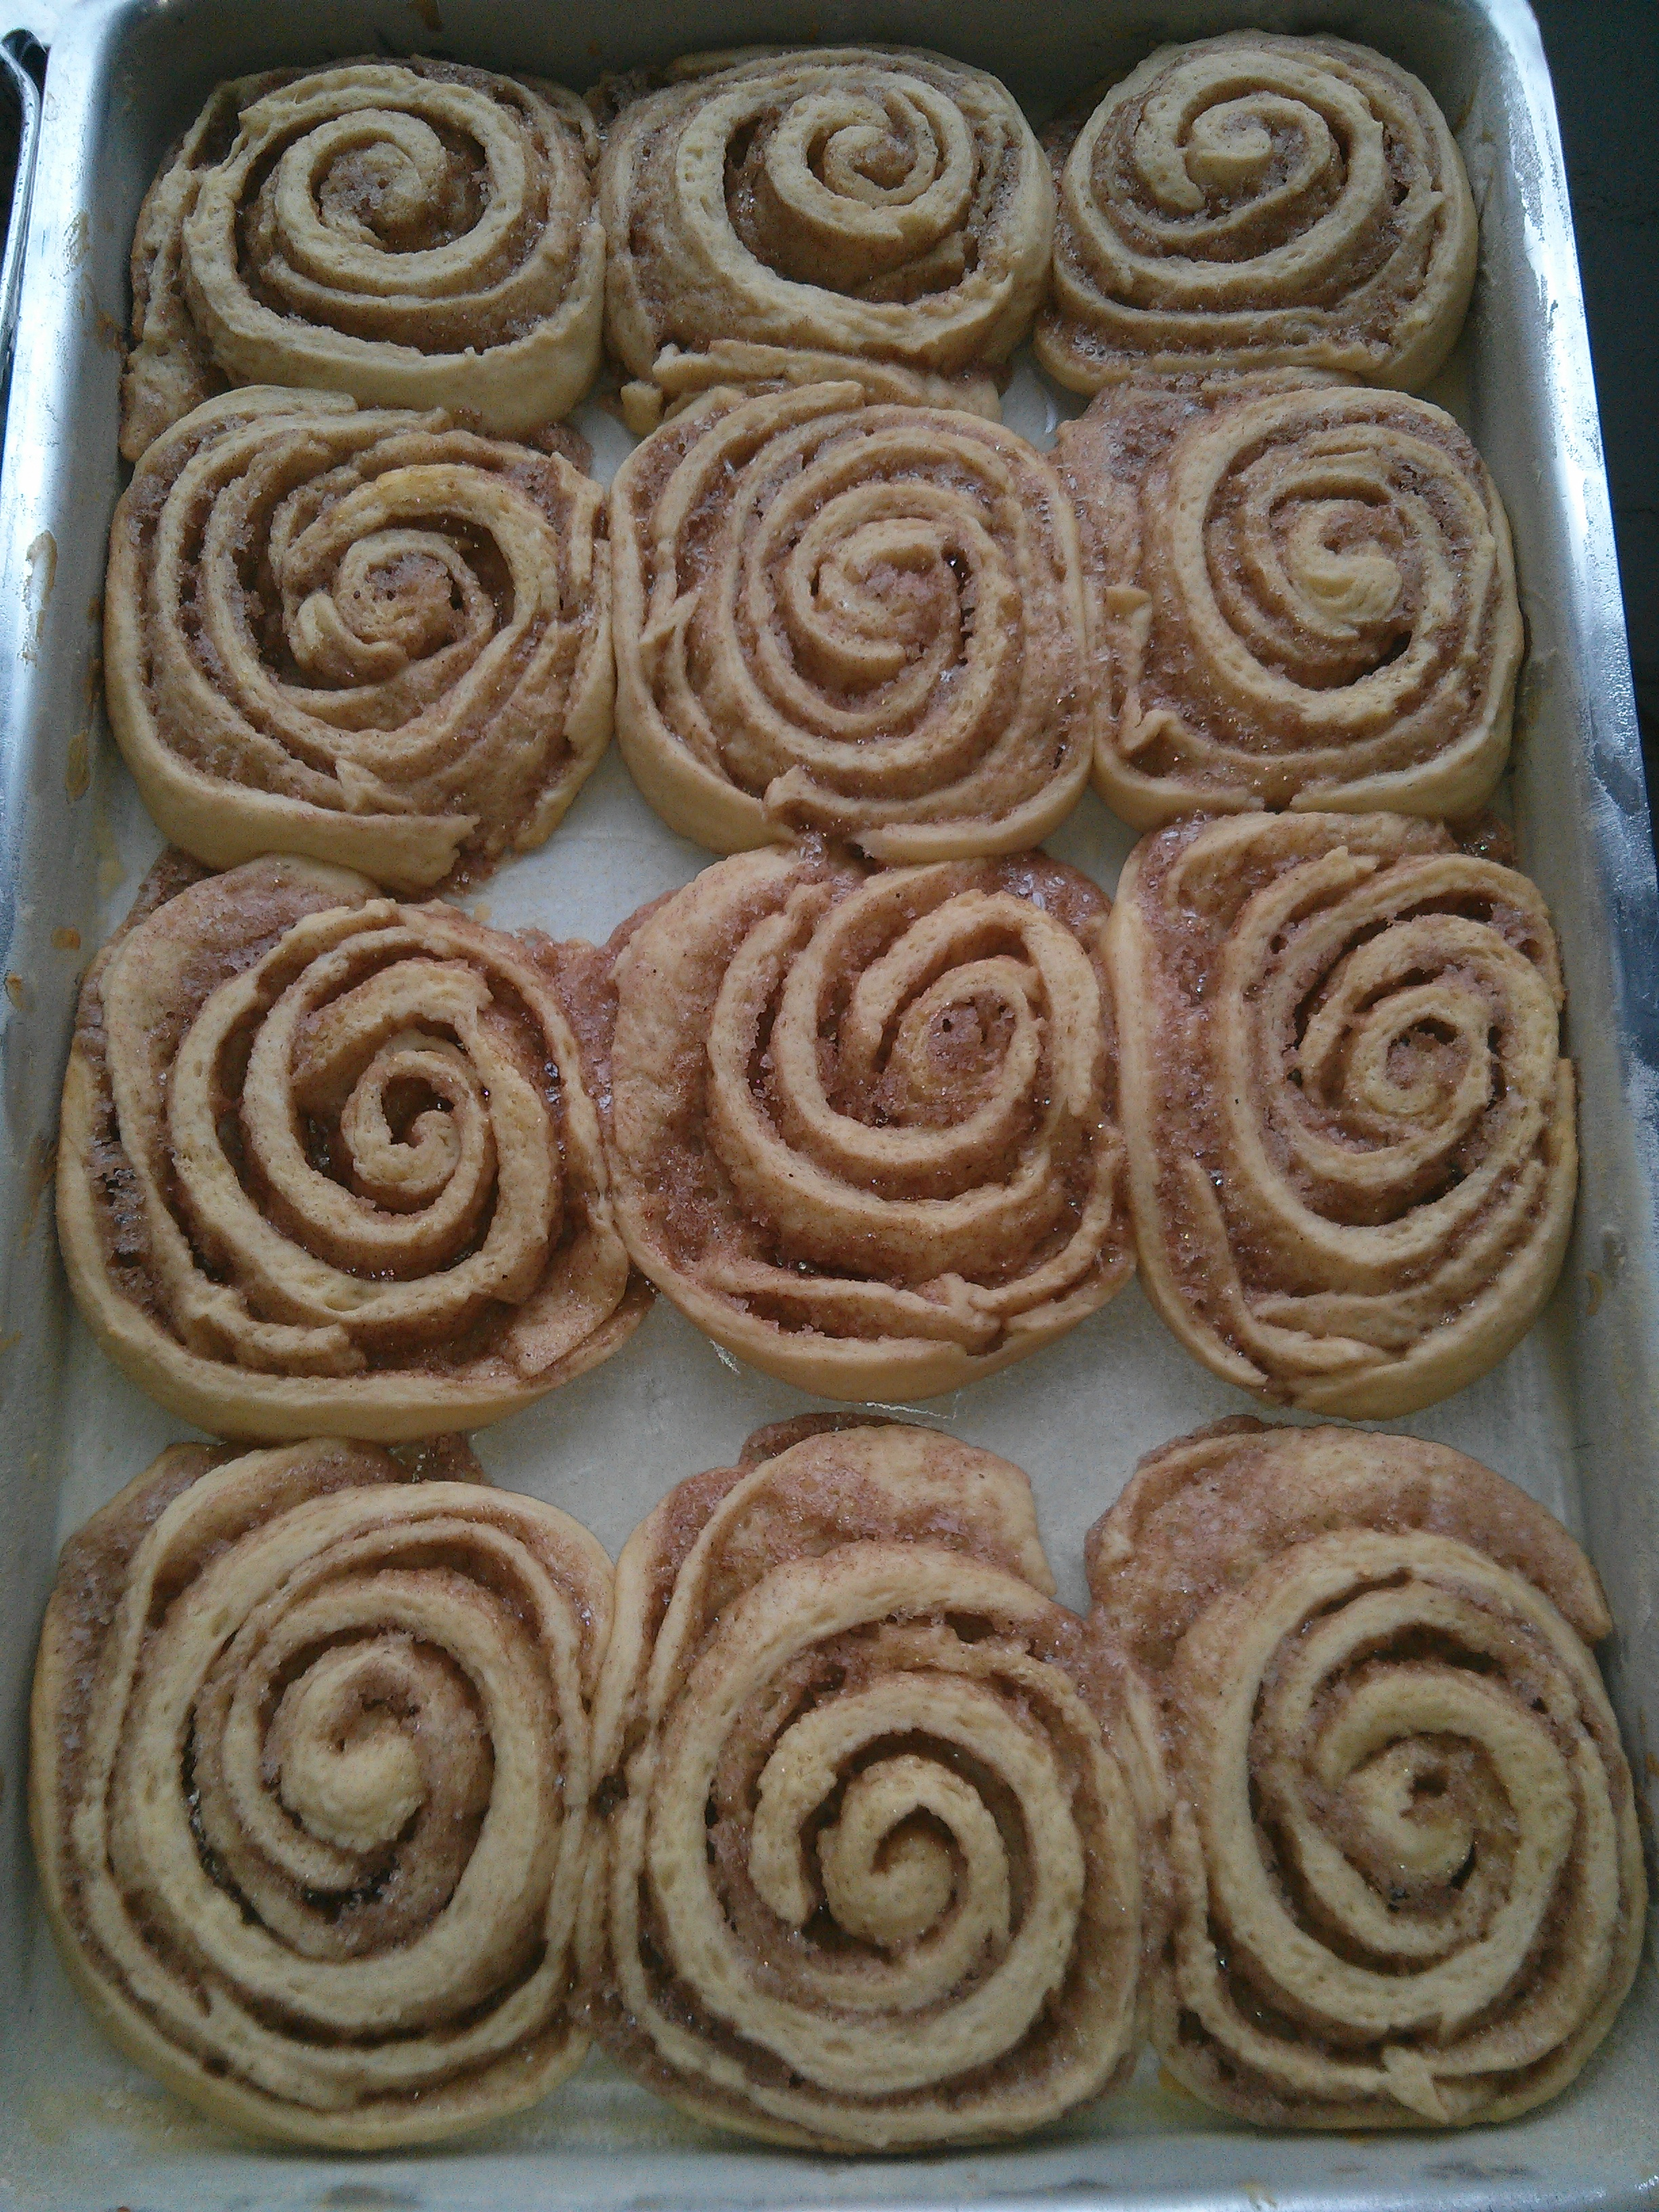
\includegraphics[height=\paperheight,width=\paperwidth]{./bilder/zimtschnecken.jpg}}
%\end{center}


%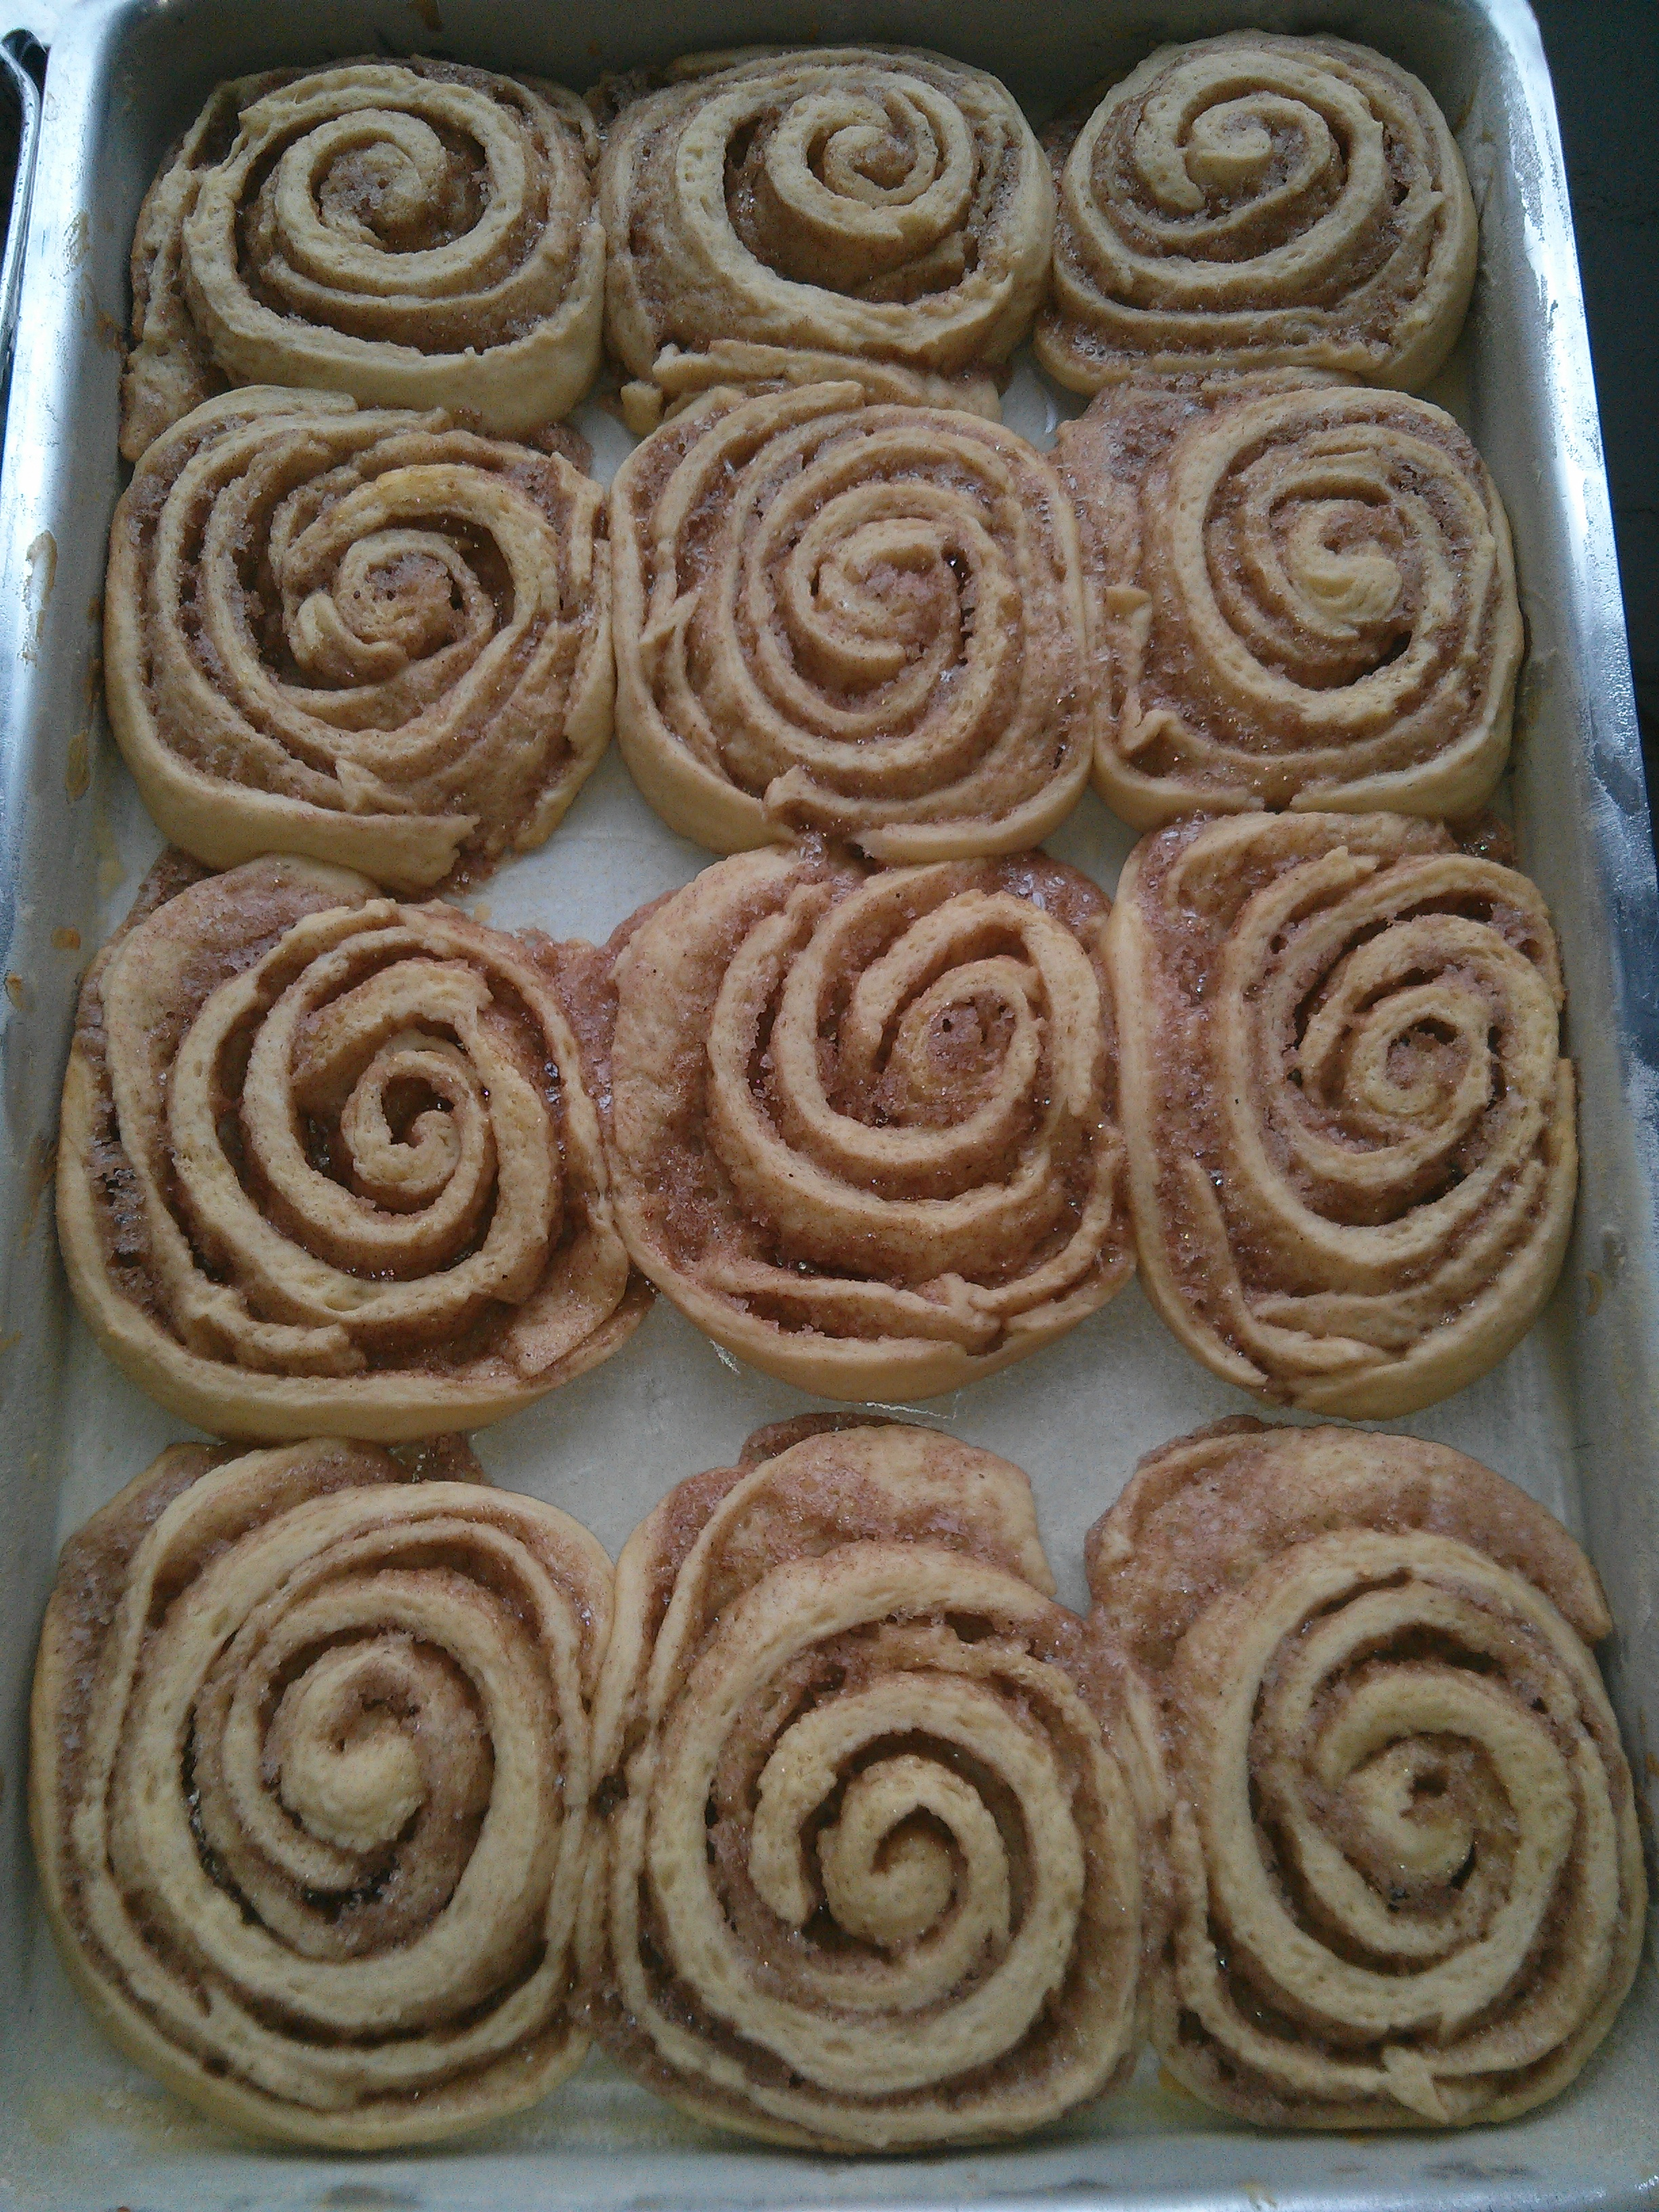
\includegraphics[width=\textwidth]{./bilder/zimtschnecken.jpg}
%\setImage{./bilder/zimtschnecken.jpg}

\begin{recipe}[]{Zimtschnecken} %Josi
	\timerecipe[Minuten]{ca. 120} %mit [EINHEIT]
	
	\personcount[Blech]{1} % mit[ART]
	\ingredient{500g Mehl}
	\ingredient{50g Hefe}
	\ingredient{250ml lauwarme Milch}
	\ingredient{270g weiche Butter}
	\ingredient{250g Zucker}
	\ingredient{0,5 TL Kardamom}
	\ingredient{2 EL Zimt}
	\ingredient{0,5 TL Salz}

\step
Die \textbf{500g Mehl} in eine Schüssel geben in einer Kuhle \textbf{250ml lauwarme Milch} und \textbf{50g Hefe} vermischen und ca. 10 min gehen lassen. 

\step
Zusammen mit \textbf{70g weiche Butter}, \textbf{0,5 TL Kardamom} und \textbf{0,5 TL Salz} zu einem Teig verkneten und 40 min gehen lassen.

\step
In der Zwischenzeit für die Füllung \textbf{200g weiche Butter}, \textbf{200g Zucker} mit \textbf{2 EL Zimt} cremig schlagen.

\step
Teig nocheinmal kräftig kneten, in zwei Teile teilen, jeweils ca. 30 cm breit ausrollen und mit der Füllungsmasse bestreichen. Die beiden Teige aufeinanderlegen und aufrollen.

\step
Die Teigrolle in ca. 3 cm breite Scheiben schneiden und diese auf einem Blech mit auslegen. Vor dem Backen nochmals 20 min gehen lassen. 

\step
Backofen vorheizen. Auf mittlerer Schiene 10 min bei 200°C und dann nochmals ca. 15 min bei 180°C backen. 

% Seite mit Bild nach dem Rezept
%\graphic{./bilder/zimtschnecken.jpg}

\tippbox{\textbf{Tipp:} Seiten der Zimtrollen vor dem Backen noch mit Eigelb einpinseln.} % Tipp in extra Rahmen

\end{recipe}

% background Image
%\tikz[remember picture,overlay] \node[opacity=0.3,inner sep=0pt] at (current page.center){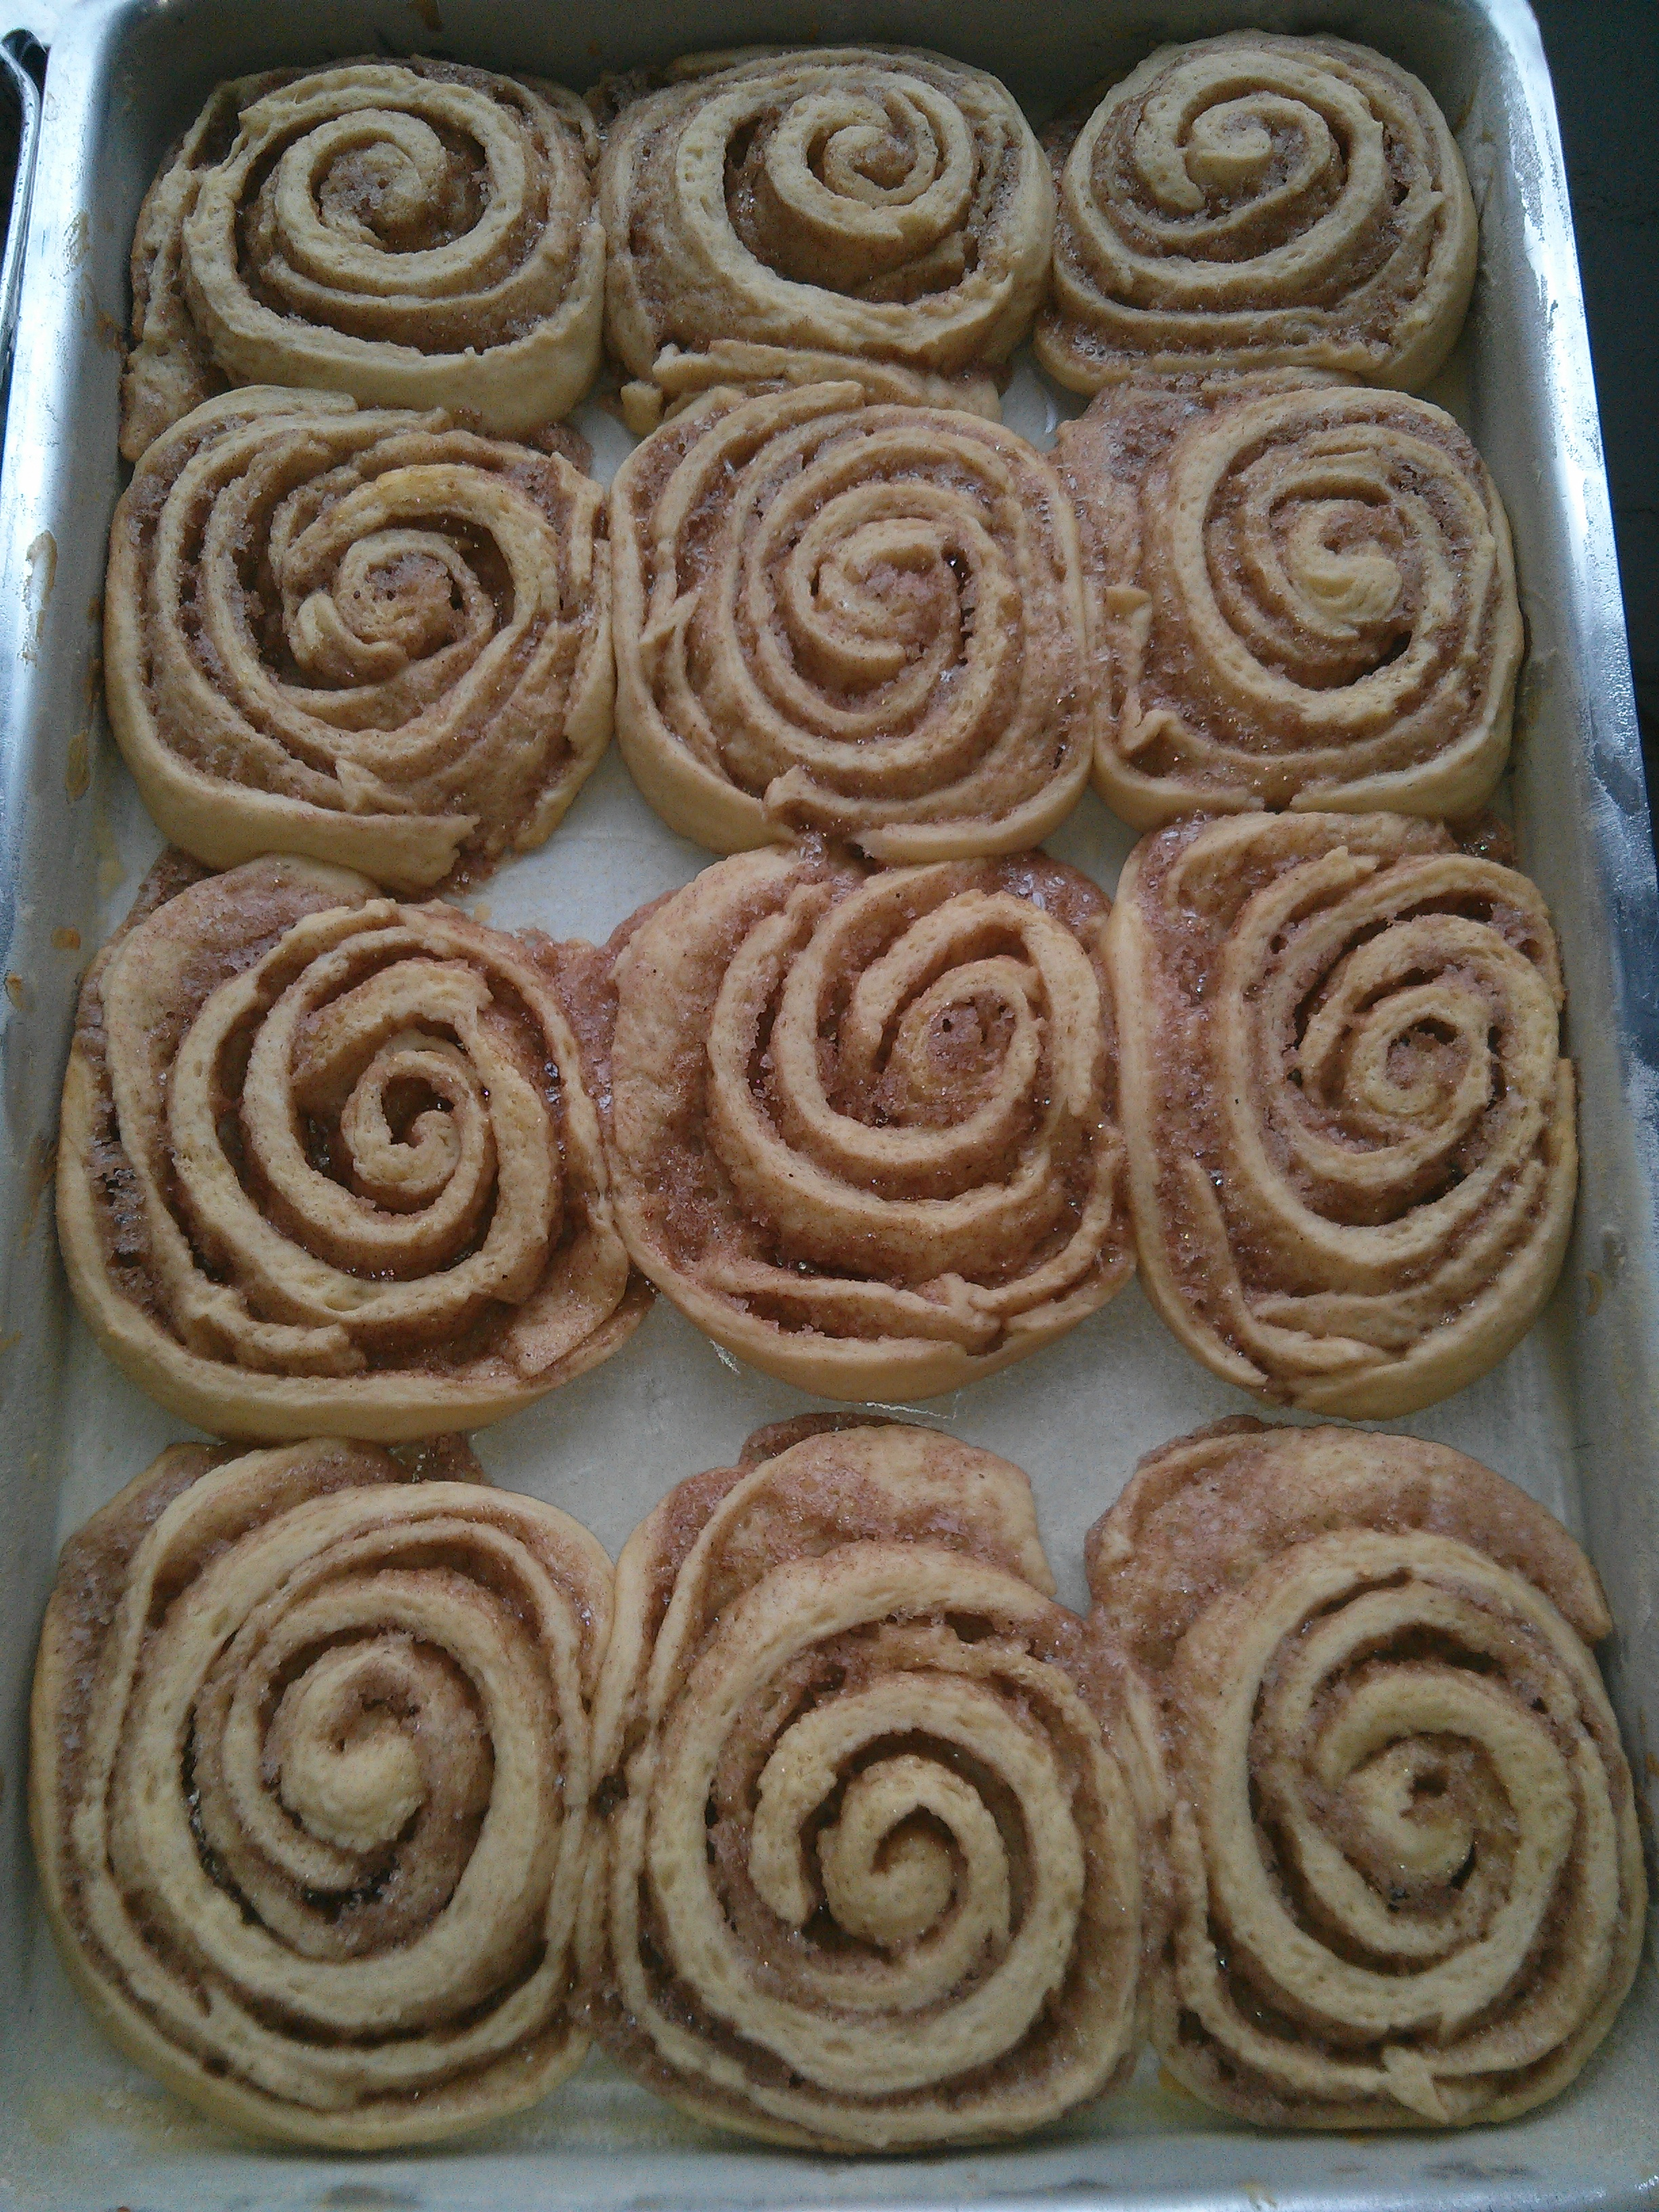
\includegraphics[width=\paperwidth,height=\paperheight]{./bilder/zimtschnecken.jpg}};

\newpage
\tikz[remember picture,overlay] \node[opacity=1,inner sep=0pt] at (current page.center){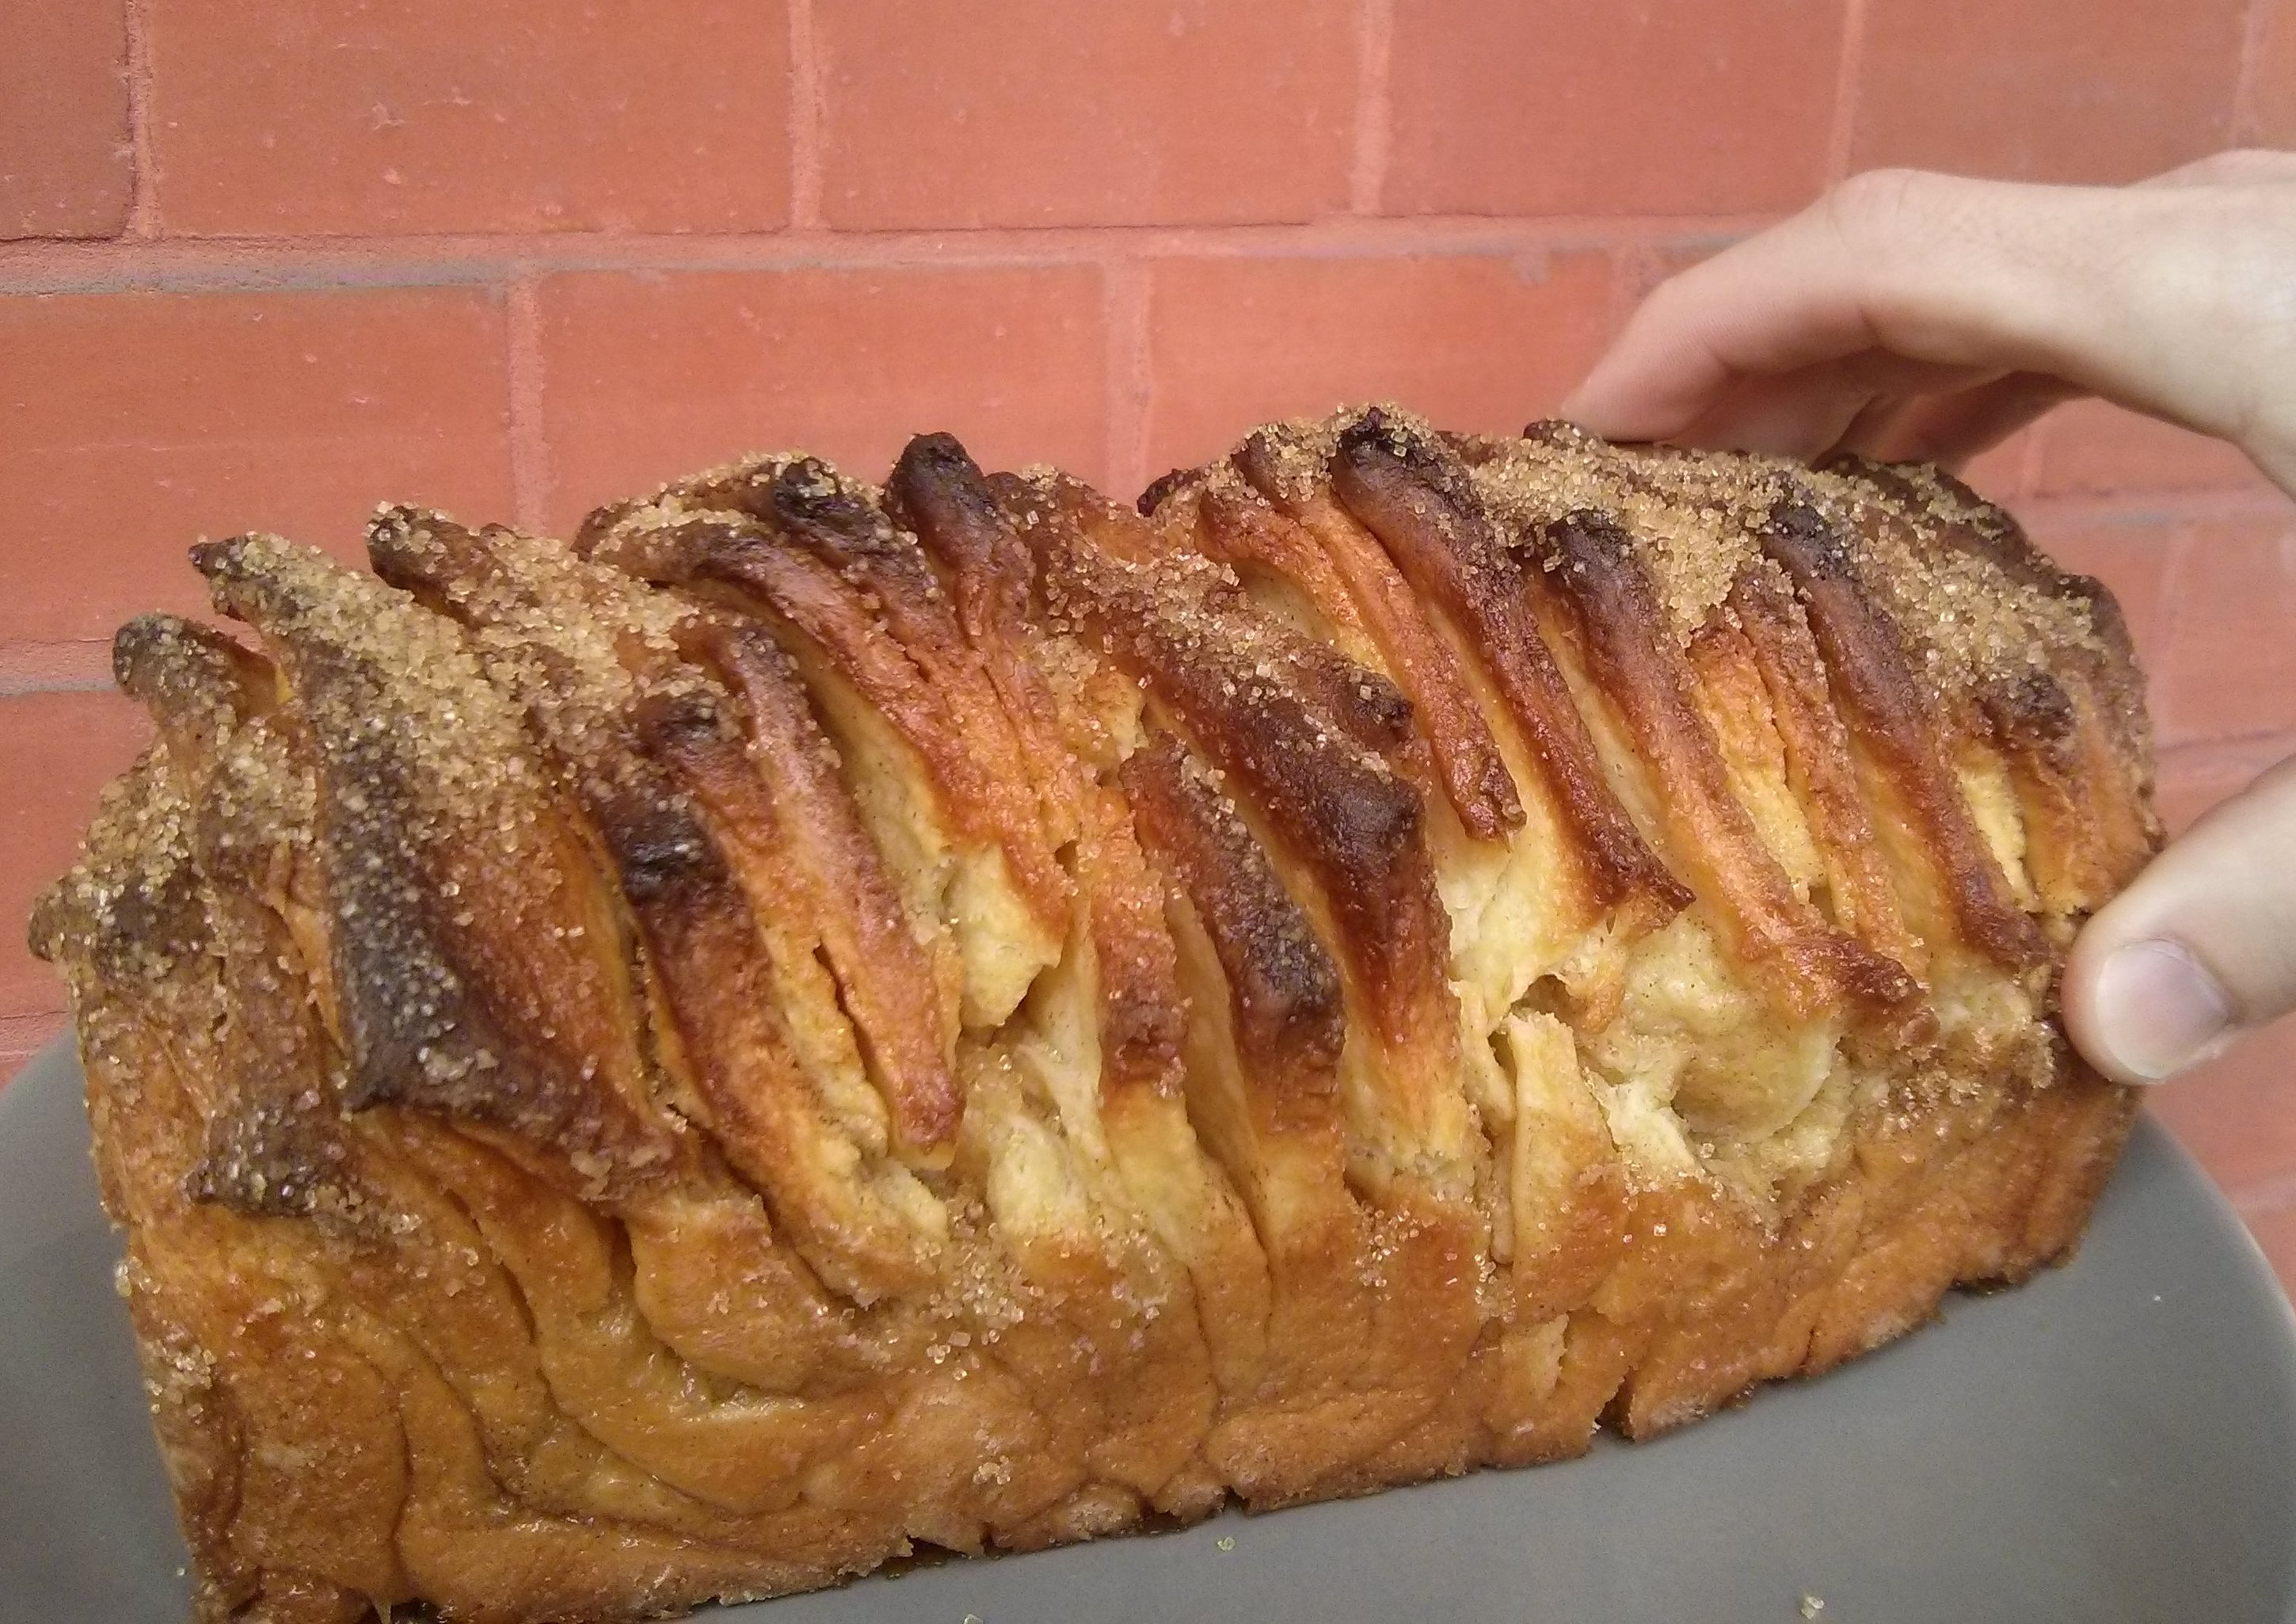
\includegraphics[width=\paperwidth,height=\paperheight]{./bilder/faltenkuchen_ratio.jpg}};

\begin{recipe}[]{Faltenkuchen} %Quelle
	\timerecipe[Minuten]{ca. 30+180+40} %mit [EINHEIT]
	\personcount[Kastenform (25 cm)]{1} % mit[ART]
	\ingredient{20g frische Hefe} % ggf. \nicefrac{1}{2}
	\ingredient{150ml lauwarme Milch}
	\ingredient{50g Zucker}
	\ingredient{1/2 TL Salz}
	\ingredient{2 Eier}
	\ingredient{375g Mehl}
	\ingredient{125g geschmolzene Butter}
	\ingredient{100g brauner Zucker}
	\ingredient{1 TL Zimt}



\step
\textbf{20g Hefe} in \textbf{150ml lauwarmer Milch} mit einigen Krümeln \textbf{Zucker} auflösen und stehen lassen bis es Blasen bildet.

\step
\textbf{50g Zucker}, \textbf{1/2 TL Salz}, \textbf{2 Eier}, \textbf{375g Mehl} und \textbf{50g geschmolzene Butter} mischen. Die Hefemasse dazu geben, kräftig mit einem Kochlöffel durchschlagen - die Masse ist ziemlich dünn, ist aber richtig so. Den Teig zugedeckt ca. 1 - 1,5 Std. gehen lassen.

\step
Den Teig auf einer bemehleten Fläche ca. 1/2 cm - 1cm dick ausrollen, danach mit einem Pinsel mit \textbf{75g geschmolzener Butter} bestreichen (1 EL von der Butter für später aufheben). \textbf{100g braunen Zucker} mit \textbf{1 TL Zimt} mischen auf dem ausgerollen Teig verteilen (1 EL von der Zimt-Zuckermischung  für später aufheben).

\step
Den Teig in der breite der Kuchenform in Streifen schneiden. Diese Streifen jetzt in der Höhe der Kuchenform in Vierecke schneiden, diese Vierecke übereinander schichten zu Paketen und in der Kastenform hintereinander setzten. Den Teig in der Form nochmals 30 Minuten gehen lassen.

\step
Im vorgeheizten Ofen bei 180 Grad auf der zweiten Schiene von unten 30-40 Minuten backen. Den noch warmen Kuchen mit einem Pinsel mit der restlichen flüssigen Butter bestreichen und mit der restlichen Zimt-Zuckermischung bestreuen. 

%\tippbox{\textbf{Tipp:} ...} % Tipp in extra Rahmen
\end{recipe}

\newpage
{\vspace*{4cm}\section{Plätzchen}}
\begin{recipe}[]{Schokoladenbrot} %Hohreins
	\timerecipe[Minuten]{ca. } %mit [EINHEIT]
	\personcount[Blech]{1} % mit[ART]
	 % ggf. \nicefrac{1}{2}
	\ingredient{250g Butter}
	\ingredient{250g Zucker}
	\ingredient{6 Eier}
	\ingredient{250g geriebene Schokolade}
	\ingredient{250g geriebene Haselnüsse}
	\ingredient{100g Mehl}
	\ingredient{1 Eßl. Rum}
	\ingredient{Schokoladenglasur}

\step
\textbf{250g Butter}, \textbf{250g Zucker} und die \textbf{6 Eier} gut verrühren.

\step
Anschließend \textbf{250g Schokolade}, \textbf{250g Haselnüsse}, \textbf{100g Mehl}, \textbf{1 Eßl. Rum},  und \textbf{eine Priese Salz} zugeben.

\step
Blech fetten und den Teig darauf verteilen.

\step
Ca. 20-30 Minuten bei 180°C Ober-Unterhitze backen.

\step
Noch heiß in Streifen schneiden und mit Schokoladenglasur überziehen.

%\tippbox{\textbf{Tipp:} ...} % Tipp in extra Rahmen
\end{recipe}
\begin{recipe}[]{Kokosmakronen} %http://www.chefkoch.de/rezepte/1513641256654130/Saftige-Kokosmakronen.html
	\timerecipe[Minuten]{ca. 15 + 10} %mit [EINHEIT]
	\personcount[Makronen]{65} % mit[ART]
	 % ggf. \nicefrac{1}{2}
	\ingredient{200g Kokosraspeln}
	\ingredient{150g Zucker}
	\ingredient{65g Quark}
	\ingredient{4 Eiweiß}
	\ingredient{1 Pck. Vanillezucker}
	\ingredient{65 Oblaten}

\step
\textbf{4 Einweiß} steif schlagen. Dann \ingredient{150g Zucker} und \ingredient{1 Pck. Vanillezucker} mit steif schlagen.

\step
\textbf{65g Quark} und \textbf{200g Kokosraspeln} unterheben.

\step
Mit Hilfe von zwei Löffeln auf die Oblaten häufen.

\step
Bei \textbf{175°C Umluft} ca. 10 - 12 Minuten backen.

%\tippbox{\textbf{Tipp:} ...} % Tipp in extra Rahmen
\end{recipe}
\begin{recipe}[]{Rosmarinkekse} %Laura
	\timerecipe[Minuten]{ca. 15 + 30 + 15} %mit [EINHEIT]
	\personcount[Kekse]{40} % mit[ART]
	 % ggf. \nicefrac{1}{2}
	\ingredient{200g Mehl}
	\ingredient{1 TL Backpulver}
	\ingredient{80g Butter}
	\ingredient{\nicefrac{1}{4} TL Salz}
	\ingredient{1 Eigelb}
	\ingredient{2 TL Rosmarin}
	\ingredient{4 EL Milch}

\step
\textbf{200g Mehl}, \textbf{1 TL Backpulver}, \textbf{80g Butter}, \textbf{\nicefrac{1}{4} TL Salz}, \textbf{1 Eigelb}, \textbf{2 TL gehackten Rosmarin} mit \textbf{2-3 EL kaltem Wasser} zu einem glatten Teig verkneten. 

\step
Den Teig in Folie wickeln und 30 Minuten im Kühlschrank kalt stellen.

\step
Den Teig ca. 5 mm dünn ausrollen und in rechteckige Kekse schneiden.

\step
Die Kekse auf dem Blech mehrmals vorsichtig mit der Gabel einstechen.

\step
Im vorgeheizten Backofen bei \textbf{200°C} etwa \textbf{12 Minuten} backen.


%\tippbox{\textbf{Tipp:} ...} % Tipp in extra Rahmen
\end{recipe}
\begin{recipe}[]{Vanillekipfel} %
	\timerecipe[Minuten]{ca. 30 + 10} %mit [EINHEIT]
	\personcount[Plätzchen]{40} % mit[ART]
	 % ggf. \nicefrac{1}{2}
	\ingredient{200g Butter}
	\ingredient{80g Zucker}
	\ingredient{100g gemahl. Nüsse}
	\ingredient{280g Mehl}
	\ingredient{125g Puderzucker}
	\ingredient{1 Pkt. Vanillezucker}


\step
\textbf{200g Butter}, \textbf{80g Zucker} und \textbf{100g gemahl. Nüsse} verrühren. Dann mit \textbf{280g Mehl} verkneten.

\step
Kleine Hörnchen formen und bei \textbf{200°C} etwa \textbf{10 Minuten} backen.

\step
\textbf{125g Puderzucker} und \textbf{1 Pkt. Vanillezucker} mischen und die Kipfel noch heiß darin wenden.

%\tippbox{\textbf{Tipp:} ...} % Tipp in extra Rahmen
\end{recipe}

\newpage
{\vspace*{4cm}\section{Getränke}}
\begin{recipe}[]{Himbeer Limes} %http://www.chefkoch.de/rezepte/510361146660274/Himbeer-Limes.html
	\timerecipe[Minuten]{ca. 30} %mit [EINHEIT]
	\personcount[Liter]{1,5} % mit[ART]
	\ingredient{500g Himbeeren} % ggf. \nicefrac{1}{2}
	\ingredient{200g Zucker}
	\ingredient{100ml Zitronensaft}
	\ingredient{200ml Wodka}
	\ingredient{100ml Himbeergeist}

\step
\textbf{200ml Wasser} erhitzen und darin \textbf{200g Zucker} lösen.

\step
\textbf{500g Himbeeren} im Mixer zerkleinern und mit \textbf{200ml Wodka}, \textbf{100ml Zitronensaft}, \textbf{100ml Himbeergeist} und dem abgekühlten Zuckerwasser mischen.

\step
In Flaschen abfüllen und kalt stellen.

%\tippbox{{\bf Tipp:} ...} % Tipp in extra Rahmen
\end{recipe}
\begin{recipe}[]{Pfirsich-Maracuja Likör} %http://www.chefkoch.de/rezepte/724061175154589/Pfirsich-Maracuja-Likoer.html
	\timerecipe[Minuten]{ca. 15} %mit [EINHEIT]
	\personcount[Liter]{2} % mit[ART]
	\ingredient{1 Liter Pfirsich-Maracuja-Saft} % ggf. \nicefrac{1}{2}
	\ingredient{2 Becher Maracuja-Joghurt}
	\ingredient{200g Zucker}
	\ingredient{1 Pk. Vanillezucker}
	\ingredient{200ml Wodka}
	\ingredient{2 Becher Sahne}
	\ingredient{(3 EL Cognac)}

\step
\textbf{1 Liter Pfirsich-Maracuja-Saft}, \textbf{2 Becher Maracuja-Joghurt} und \textbf{200g Zucker} mit dem Stabmixer pürieren.

\step
\textbf{1 Pk. Vanillezucker}, \textbf{200ml Wodka}, \textbf{2 Becher Sahne} und ggf. \textbf{3 EL Cognac} dazu rühren.

\step
In Flaschen abfüllen und kalt stellen.

%\tippbox{{\bf Tipp:} ...} % Tipp in extra Rahmen
\end{recipe}

\end{document}

%\begin{recipe}{}
%	\timerecipe{ca. $1\frac{1}{4}$}
%	\personcount{4-6}
%	\ingredient{}
%
%\step
%
%\end{recipe}
